% Created 2024-05-12 Sun 12:25
% Intended LaTeX compiler: pdflatex
\documentclass[energies,article,submit,moreauthors]{Definitions/mdpi}

%--------------------
% Class Options:
%--------------------
%----------
% journal
%----------
% Choose between the following MDPI journals:
% acoustics, actuators, addictions, admsci, adolescents, aerobiology, aerospace, agriculture, agriengineering, agrochemicals, agronomy, ai, air, algorithms, allergies, alloys, analytica, analytics, anatomia, animals, antibiotics, antibodies, antioxidants, applbiosci, appliedchem, appliedmath, applmech, applmicrobiol, applnano, applsci, aquacj, architecture, arm, arthropoda, arts, asc, asi, astronomy, atmosphere, atoms, audiolres, automation, axioms, bacteria, batteries, bdcc, behavsci, beverages, biochem, bioengineering, biologics, biology, biomass, biomechanics, biomed, biomedicines, biomedinformatics, biomimetics, biomolecules, biophysica, biosensors, biotech, birds, bloods, blsf, brainsci, breath, buildings, businesses, cancers, carbon, cardiogenetics, catalysts, cells, ceramics, challenges, chemengineering, chemistry, chemosensors, chemproc, children, chips, cimb, civileng, cleantechnol, climate, clinpract, clockssleep, cmd, coasts, coatings, colloids, colorants, commodities, compounds, computation, computers, condensedmatter, conservation, constrmater, cosmetics, covid, crops, cryptography, crystals, csmf, ctn, curroncol, cyber, dairy, data, ddc, dentistry, dermato, dermatopathology, designs, devices, diabetology, diagnostics, dietetics, digital, disabilities, diseases, diversity, dna, drones, dynamics, earth, ebj, ecologies, econometrics, economies, education, ejihpe, electricity, electrochem, electronicmat, electronics, encyclopedia, endocrines, energies, eng, engproc, entomology, entropy, environments, environsciproc, epidemiologia, epigenomes, est, fermentation, fibers, fintech, fire, fishes, fluids, foods, forecasting, forensicsci, forests, foundations, fractalfract, fuels, future, futureinternet, futurepharmacol, futurephys, futuretransp, galaxies, games, gases, gastroent, gastrointestdisord, gels, genealogy, genes, geographies, geohazards, geomatics, geosciences, geotechnics, geriatrics, grasses, gucdd, hazardousmatters, healthcare, hearts, hemato, hematolrep, heritage, higheredu, highthroughput, histories, horticulturae, hospitals, humanities, humans, hydrobiology, hydrogen, hydrology, hygiene, idr, ijerph, ijfs, ijgi, ijms, ijns, ijpb, ijtm, ijtpp, ime, immuno, informatics, information, infrastructures, inorganics, insects, instruments, inventions, iot, j, jal, jcdd, jcm, jcp, jcs, jcto, jdb, jeta, jfb, jfmk, jimaging, jintelligence, jlpea, jmmp, jmp, jmse, jne, jnt, jof, joitmc, jor, journalmedia, jox, jpm, jrfm, jsan, jtaer, jvd, jzbg, kidneydial, kinasesphosphatases, knowledge, land, languages, laws, life, liquids, literature, livers, logics, logistics, lubricants, lymphatics, machines, macromol, magnetism, magnetochemistry, make, marinedrugs, materials, materproc, mathematics, mca, measurements, medicina, medicines, medsci, membranes, merits, metabolites, metals, meteorology, methane, metrology, micro, microarrays, microbiolres, micromachines, microorganisms, microplastics, minerals, mining, modelling, molbank, molecules, mps, msf, mti, muscles, nanoenergyadv, nanomanufacturing,\gdef\@continuouspages{yes}} nanomaterials, ncrna, ndt, network, neuroglia, neurolint, neurosci, nitrogen, notspecified, %%nri, nursrep, nutraceuticals, nutrients, obesities, oceans, ohbm, onco, %oncopathology, optics, oral, organics, organoids, osteology, oxygen, parasites, parasitologia, particles, pathogens, pathophysiology, pediatrrep, pharmaceuticals, pharmaceutics, pharmacoepidemiology,\gdef\@ISSN{2813-0618}\gdef\@continuous pharmacy, philosophies, photochem, photonics, phycology, physchem, physics, physiologia, plants, plasma, platforms, pollutants, polymers, polysaccharides, poultry, powders, preprints, proceedings, processes, prosthesis, proteomes, psf, psych, psychiatryint, psychoactives, publications, quantumrep, quaternary, qubs, radiation, reactions, receptors, recycling, regeneration, religions, remotesensing, reports, reprodmed, resources, rheumato, risks, robotics, ruminants, safety, sci, scipharm, sclerosis, seeds, sensors, separations, sexes, signals, sinusitis, skins, smartcities, sna, societies, socsci, software, soilsystems, solar, solids, spectroscj, sports, standards, stats, std, stresses, surfaces, surgeries, suschem, sustainability, symmetry, synbio, systems, targets, taxonomy, technologies, telecom, test, textiles, thalassrep, thermo, tomography, tourismhosp, toxics, toxins, transplantology, transportation, traumacare, traumas, tropicalmed, universe, urbansci, uro, vaccines, vehicles, venereology, vetsci, vibration, virtualworlds, viruses, vision, waste, water, wem, wevj, wind, women, world, youth, zoonoticdis
% For posting an early version of this manuscript as a preprint, you may use "preprints" as the journal. Changing "submit" to "accept" before posting will remove line numbers.

%---------
% article
%---------
% The default type of manuscript is "article", but can be replaced by:
% abstract, addendum, article, book, bookreview, briefreport, casereport, comment, commentary, communication, conferenceproceedings, correction, conferencereport, entry, expressionofconcern, extendedabstract, datadescriptor, editorial, essay, erratum, hypothesis, interestingimage, obituary, opinion, projectreport, reply, retraction, review, perspective, protocol, shortnote, studyprotocol, systematicreview, supfile, technicalnote, viewpoint, guidelines, registeredreport, tutorial
% supfile = supplementary materials

%----------
% submit
%----------
% The class option "submit" will be changed to "accept" by the Editorial Office when the paper is accepted. This will only make changes to the frontpage (e.g., the logo of the journal will get visible), the headings, and the copyright information. Also, line numbering will be removed. Journal info and pagination for accepted papers will also be assigned by the Editorial Office.

%------------------
% moreauthors
%------------------
% If there is only one author the class option oneauthor should be used. Otherwise use the class option moreauthors.

%---------
% pdftex
%---------
% The option pdftex is for use with pdfLaTeX. Remove "pdftex" for (1) compiling with LaTeX & dvi2pdf (if eps figures are used) or for (2) compiling with XeLaTeX.

%=================================================================
% MDPI internal commands - do not modify
\firstpage{1}
\makeatletter
\setcounter{page}{\@firstpage}
\makeatother
\pubvolume{1}
\issuenum{1}
\articlenumber{0}
\pubyear{2024}
\copyrightyear{2024}
%\externaleditor{Academic Editor: Firstname Lastname}
\datereceived{ }
\daterevised{ } % Comment out if no revised date
\dateaccepted{ }
\datepublished{ }
%\datecorrected{} % For corrected papers: "Corrected: XXX" date in the original paper.
%\dateretracted{} % For corrected papers: "Retracted: XXX" date in the original paper.
\hreflink{https://doi.org/} % If needed use \linebreak
%\doinum{}
%\pdfoutput=1 % Uncommented for upload to arXiv.org
%\CorrStatement{yes}  % For updates


%=================================================================
% Add packages and commands here. The following packages are loaded in our class file: fontenc, inputenc, calc, indentfirst, fancyhdr, graphicx, epstopdf, lastpage, ifthen, float, amsmath, amssymb, lineno, setspace, enumitem, mathpazo, booktabs, titlesec, etoolbox, tabto, xcolor, colortbl, soul, multirow, microtype, tikz, totcount, changepage, attrib, upgreek, array, tabularx, pbox, ragged2e, tocloft, marginnote, marginfix, enotez, amsthm, natbib, hyperref, cleveref, scrextend, url, geometry, newfloat, caption, draftwatermark, seqsplit
% cleveref: load \crefname definitions after \begin{document}

%=================================================================
% Please use the following mathematics environments: Theorem, Lemma, Corollary, Proposition, Characterization, Property, Problem, Example, ExamplesandDefinitions, Hypothesis, Remark, Definition, Notation, Assumption
%% For proofs, please use the proof environment (the amsthm package is loaded by the MDPI class).

%=================================================================
% Full title of the paper (Capitalized)
\Title{A Simulated Annealing Approach to the Scheduling of Battery-Electric Bus Charging}

% MDPI internal command: Title for citation in the left column
\TitleCitation{A Simulated Annealing Approach to the Scheduling of Battery-Electric Bus Charging}

% Author Orchid ID: enter ID or remove command
%\newcommand{\orcidauthorA}{0000-0000-0000-000X} % Add \orcidA{} behind the author's name
%\newcommand{\orcidauthorB}{0000-0000-0000-000X} % Add \orcidB{} behind the author's name

% Authors, for the paper (add full first names)
\Author{Alexander Brown$^{1,\dagger,}$* and Greg Droge$^{2,\dagger,\ddagger}$}

%\longauthorlist{yes}

% MDPI internal command: Authors, for metadata in PDF
\AuthorNames{Alexander Brown and Greg Droge}

% MDPI internal command: Authors, for citation in the left column
\AuthorCitation{Brown, A.; Droge G.}
% If this is a Chicago style journal: Lastname, Firstname, Firstname Lastname, and Firstname Lastname.

% Affiliations / Addresses (Add [1] after \address if there is only one affiliation.)
\address{%
$^{1}$ \quad Utah State University; a01704744@usu.edu\\
$^{2}$ \quad Utah State University; greg.droge@usu.edu}

% Contact information of the corresponding author
\corres{Correspondence: a01704744@usu.edu}

% Current address and/or shared authorship
\firstnote{Current address: 102 Old Main Hl, Logan, UT 84322-0102.}  % Current address should not be the same as any items in the Affiliation section.
\secondnote{These authors contributed equally to this work.}
% The commands \thirdnote{} till \eighthnote{} are available for further notes

%\simplesumm{} % Simple summary

%\conference{} % An extended version of a conference paper

% The fields PACS, MSC, and JEL may be left empty or commented out if not applicable
%\PACS{J0101}
%\MSC{}
%\JEL{}

%%%%%%%%%%%%%%%%%%%%%%%%%%%%%%%%%%%%%%%%%%
% Only for the journal Diversity
%\LSID{\url{http://}}

%%%%%%%%%%%%%%%%%%%%%%%%%%%%%%%%%%%%%%%%%%
% Only for the journal Applied Sciences
%\featuredapplication{Authors are encouraged to provide a concise description of the specific application or a potential application of the work. This section is not mandatory.}
%%%%%%%%%%%%%%%%%%%%%%%%%%%%%%%%%%%%%%%%%%

%%%%%%%%%%%%%%%%%%%%%%%%%%%%%%%%%%%%%%%%%%
% Only for the journal Data
%\dataset{DOI number or link to the deposited data set if the data set is published separately. If the data set shall be published as a supplement to this paper, this field will be filled by the journal editors. In this case, please submit the data set as a supplement.}
%\datasetlicense{License under which the data set is made available (CC0, CC-BY, CC-BY-SA, CC-BY-NC, etc.)}

%%%%%%%%%%%%%%%%%%%%%%%%%%%%%%%%%%%%%%%%%%
% Only for the journal Toxins
%\keycontribution{The breakthroughs or highlights of the manuscript. Authors can write one or two sentences to describe the most important part of the paper.}

%%%%%%%%%%%%%%%%%%%%%%%%%%%%%%%%%%%%%%%%%%
% Only for the journal Encyclopedia
%\encyclopediadef{For entry manuscripts only: please provide a brief overview of the entry title instead of an abstract.}

%%%%%%%%%%%%%%%%%%%%%%%%%%%%%%%%%%%%%%%%%%
% Only for the journal Advances in Respiratory Medicine
%\addhighlights{yes}
%\renewcommand{\addhighlights}{%

%\noindent This is an obligatory section in “Advances in Respiratory Medicine”, whose goal is to increase the discoverability and readability of the article via search engines and other scholars. Highlights should not be a copy of the abstract, but a simple text allowing the reader to quickly and simplified find out what the article is about and what can be cited from it. Each of these parts should be devoted up to 2~bullet points.\vspace{3pt}\\
%\textbf{What are the main findings?}
% \begin{itemize}[labelsep=2.5mm,topsep=-3pt]
% \item First bullet.
% \item Second bullet.
% \end{itemize}\vspace{3pt}
%\textbf{What is the implication of the main finding?}
% \begin{itemize}[labelsep=2.5mm,topsep=-3pt]
% \item First bullet.
% \item Second bullet.
% \end{itemize}
%}

\usepackage{subcaption}                     % Subfigures
\usepackage[ruled]{algorithm2e}             % Algorithms
\usepackage{listings}                       % Code in LaTeX
\usepackage{listings-rust}                  % Code in LaTeX
\usepackage{amsfonts}                       % Cool math fonts
\usepackage{tabularx}                       % Cool tables
\usepackage{multicol}                       % Add capability to make columns
\usepackage[group-separator={,}, group-minimum-digits=3]{siunitx}   % Format numbers
\usepackage{soul}                           % Highlight text
\usepackage[stable]{footmisc}               % Allow footnotes in section headers
\setlength\parindent{0pt}                   % No indent for paragraphs
\usepackage{xfp}                             % No trailing zeros
\lstset{language=Rust, style=boxed}
\usetikzlibrary{arrows.meta}                % Arrows for tikz
\newcommand{\definitionautorefname}{Definition}
\newcommand{\Or}{\textbf{ or }}
\renewcommand*{\And}{\textbf{ and }}
\newcolumntype{L}[1]{>{\hsize=#1\hsize\raggedright\arraybackslash}X}%
\newcommand{\mathcolorbox}[1]{\colorbox{yellow}{$\displaystyle #1$}}
\newcommand\mysubcaption[1]{\phantomcaption%
\caption*{\figurename~\thefigure(\thesubfigure). #1}}
\newcommand\mycommfont[1]{\footnotesize\ttfamily\textcolor{gray}{#1}}
\newcommand{\T}{\mathcal{T}}                % To make it clear the difference
\newcommand{\Tau}{T}                        % between Tau and T
\newcommand{\AC}{AC(u, d, v, \eta)}         % Set the parameters for AC once
\newcommand{\UC}{UC(u, d, v)}               % Set the parameters for UC once
\newcommand{\ACi}{AC(u_i, d_i, q_i, \eta_i)}% Set the parameters for AC once
\newcommand{\UCi}{UC(u_i, d_i, q_i)}        % Set the parameters for UC once
\newcommand{\Not}{\textbf{not }}            % Custom `not' operator
\newcommand{\visit}{(i, b, a, e, u, d, q, \eta, \xi)}
\newcommand{\I}{\mathbb{I}}                 % Set of visit tuples
\newcommand{\C}{\mathbb{C}}                 % Charger availability information
\newcommand{\U}{\mathcal{U}}                % Uniform distribution
\newcommand{\W}{\mathcal{W}}                % Weighted distribution
\newcommand{\Sol}{\mathbb{S}}               % A shorthand for visit tuple
\newcommand{\M}{\mathbb{M}}                 % A shorthand for the metadata
\newcommand{\Hd}{\mathbb{H}}                % Set of discrete times
\newcommand{\Nu}{\mathcal{V}}               % Draw a nice Nu
\newcommand{\Iset}{I}                       % Set of visits 1-I
\newcommand{\Isetinit}{I_0}                 % Set of visits inital visits
\newcommand{\Isetfinal}{I_f}                % Set of visits final visits
\newcommand{\Bset}{B}                       % Set of visits 1-B
\newcommand{\Qset}{Q}                       % Set of visits 1-Q
\newcommand{\Jset}{J}                       % Set of visits 1-J
\newcommand{\Jsetq}{\mathbb{J}}             % Set of visits 1-J for queue active times
\newcommand{\Hset}{H}                       % Set of visits 1-H
%%-------------------------------------------------------------------------------
% Experiment parameters
\newcommand{\A}{35 }                                                            % Number of buses
\newcommand{\N}{338 }                                                           % Number of visits
\newcommand{\Cgain}{5000}                                                       % Gain applied to penalty method
\newcommand{\acharge}{0.9}                                                      % BOD charge percentage
\newcommand{\bcharge}{0.7 }                                                     % EOD charge percentage
\newcommand{\mincharge}{25\% }                                                  % Min visit charge percent
\newcommand{\minchargeD}{0.25 }                                                 % Min visit charge decimal
\newcommand{\maxcharge}{100\% }                                                 % Max visit charge percent
\newcommand{\batsize}{388 }                                                     % Battery capacity
\newcommand{\fast}{15 }                                                         % Number of fast chargers
\newcommand{\slow}{15 }                                                         % Number of slow chargers
\newcommand{\fasts}{911 }                                                       % Speed of fast charger
\newcommand{\slows}{30 }                                                        % Speed of slow charger
\newcommand{\contvars}{7,511 }
\newcommand{\intvars}{328,282 }
\newcommand{\localcnt}{500 }                                                    % Number of local search iterations
\newcommand{\tempinit}{9000 }                                                   % Initial temperature
\newcommand{\tempcnt}{3832 }                                                    % Number of steps in temperature
\newcommand{\quicklocal}{0.4 }                                                  % Time to finish local quick
\newcommand{\heuristiclocal}{0.5 }                                              % Time to finish local heuristic
%%-------------------------------------------------------------------------------
%% Solve output
%% Solve output
\newcommand{\timeran}{4.2 }                                                    % Time ran for MILP [s]
% Abstract (Do not insert blank lines, i.e. \\)
\abstract{With an increasing adoption of Battery Electric Bus (BEB) fleets, developing a reliable charging schedule is vital to a successful migration from their fossil fuel counterparts. In this paper, a Simulated Annealing (SA) implementation is developed for a charge scheduling framework for a fixed-schedule fleet of BEBs that utilizes a proportional battery dynamics model, accounts for multiple charger types, allows partial charging, and further considers the total energy consumed by the schedule as well as peak power use. Two generation mechanisms are implemented for the SA algorithm denoted as the "quick" and "heuristic" implementations, respectively. The model validity is demonstrated by utilizing a set of routes sampled form the Utah Transit Authority (UTA) and comparing the results againts two other models: the BPAP and the Qin-Modified. The results presented show that both SA techniques offer a means of generating oprationally feasible schedules quickly while minimizing the cost of operation and considering battery health. The heuristic technique, hower, shows a quicker rate of convergence.}

% Keywords
\keyword{Battery Electric Bus (BEB), Charge Scheduling, Simulated Annealing, Position Allocation Problem (PAP), Mixed Integer Linear Program (MILP)}
\author{Alexander Brown}
\date{\today}
\title{A Simulated Annealing Approach to the Scheduling of Battery-Electric Bus Charging}
\begin{document}

\maketitle
\tableofcontents

\parskip 3mm                                % Set the vetical space between paragraphs
\let\ref\autoref                            % Redifine `\ref` as `\autoref` because lazy
\SetCommentSty{mycommfont}                  % Set the comment color

\renewcommand{\chapterautorefname}{Chapter}
\renewcommand{\sectionautorefname}{Section}
\renewcommand{\subsectionautorefname}{Section}
\renewcommand{\subsubsectionautorefname}{Section}
\renewcommand{\paragraphautorefname}{Section}
\renewcommand{\algorithmautorefname}{Algorithm}

\section{Introduction}
\label{sec:sa-introduction}
With an ever-increasing interest in the electrification of vehicles in the push for green transportation, many
organizations and companies have been looking to adopt a fleet of electric vehicles \cite{khan-2022-inves}. This
transition is also stemming into the electrification of public bus transportation via battery power, i.e., battery
electric buses (BEBs) \cite{li-2016-batter-elect,guida-2017-zeeus-repor-europ}. In particular, agencies such as the
Utah Transit Authority (UTA) have directed focus in replacing their fleets with BEBs. Alongside all the benefits that
are associated with BEBs come new challenges that must be addressed prior to their integration into mainstream
utilization. The energy storage capacity of BEBs is typically significantly less than their combustion counterparts
while also having significantly longer refueling periods \cite{xylia-2018-role-charg,li-2016-batter-elect}. This is
further complicated due to the care that must be taken in prolonging the lifespan of the battery
\cite{lutsey-2019-updat-elect,edge-2021-lithium,millner-2010-model-lithium}. As another complication, BEB refueling
is not a fixed cost (i.e. price per gallon multiplied by tank size). Utility companies, in addition to charging for the
total energy consumed over a pay period, often charge a demand cost. The demand cost is based on the peak power drawn
during the pay period and can significantly impact the overall monetary cost of maintaining the BEBs. This work
introduces a scheduling framework for a fleet of BEBs that minimizes charging costs while considering other constraints
pertinent for operation.

Works concerning charge planning often use a version of the vehicle scheduling problem \cite{zhang-2021-optim-elect,duan-2021-refor-mixed,rinaldi-2020-mixed-fleet,tang-2019-robus-sched,li-2014-trans-bus,he-2020-optim-charg},
while others have based their implementation on alternative methods
\cite{qarebagh-2019-optim-sched,whitaker-2023-a-network}. \cite{whitaker-2023-a-network} utilizes a network flow
approach to model the scheduling while \cite{qarebagh-2019-optim-sched} utilizes what is known as the Position
Allocation Problem (PAP). The vehicle scheduling problem and the work of \cite{whitaker-2023-a-network} involve the
discretization of the time horizon, whereas the PAP models the charge durations in a continuous manner reducing the
variable count. Regardless of the method utilized, nearly all the literature reviewed considers consumption costs
\cite{jahic-2019-preem,frendo-2021-open-sourc,qin-2016-numer-analy,zhou-2020-bi-objec,duan-2021-refor-mixed,mortensen-2023-cost-minim,zhou-2020-collab-optim,rinaldi-2020-mixed-fleet,zhou-2020-collab-optim}, while fewer
consider demand costs \cite{jahic-2019-preem,frendo-2021-open-sourc,qin-2016-numer-analy,mortensen-2023-cost-minim,he-2020-optim-charg}. Many of these works introduce simplifying assumptions for the sake of
computation. For example, some approaches only consider fast chargers during planing \cite{zhou-2020-collab-optim,li-2014-trans-bus,wang-2017-optim-rechar,sebastiani-2016-evaluat-elect,wei-2018-optim-spatio}. Approaches that
consider more than one charger type typically isolate the specific charger types in different locations
\cite{tang-2019-robus-sched,he-2020-optim-charg}.

When considering battery charging, some works assume that BEBs always charge to full capacity
\cite{duan-2021-refor-mixed,zhang-2021-optim-elect,zhou-2020-bi-objec,wang-2017-elect-vehic}, partial charging
utilizing a linear battery dynamics model \cite{wei-2018-optim-spatio,he-2020-optim-charg,mortensen-2023-cost-minim}, or non-linear battery dynamics with partial charging \cite{whitaker-2023-a-network,zhang-2021-optim-elect,qin-2016-numer-analy,jahic-2019-preem,frendo-2021-open-sourc}. Works that assume scheduled
BEBs always charge to full capacity significantly simplify the scheduling problem, but eliminates the key factor in
reducing the demand cost, partial charging \cite{tang-2019-robus-sched,duan-2021-refor-mixed,rinaldi-2020-mixed-fleet,zhou-2020-collab-optim}.

The selected model for the battery charge dynamics, although pertinent to this work as it directly affects the quality
of the produced schedule, does not impact the considerations of battery health. Battery health begins to be of concern
when over-charging, under-charging, utilizing fast chargers extensively, or forcing the battery to perform ``deep'' cycles
\cite{zhou-2020-bi-objec,millner-2010-model-lithium,edge-2021-lithium}. Furthermore, other works have suggested
that charging a battery nearly to capacity is detrimental to the health and can significantly reduce the total charge
cycles a battery may undergo \cite{edge-2021-lithium,millner-2010-model-lithium}. Thus, this work assumes that a
linear model is sufficiently accurate to produce an operationally valid schedule while maintaining battery health.

In respect to the state of the art provided, this work aims to expand on the PAP by introducing a Simulated Annealing
(SA) framework that utilizes a proportional battery dynamics model, considers battery health by encouraging slow charger
use, allows for partial charging, allows for multiple charger types, minimizes consumption cost, and minimizes demand
cost. These contributions are demonstrated via simulation and comparison to two other models: an implementation of the
PAP for BEBs, denoted as BPAP, and what is known as the Qin-Modified technique.

The remainder of this paper goes as follows. \ref{sec:sa-problem-description} provides the problem statement associated with
this work. \ref{sec:sa-optimization-problem} provides a description of the input parameters and decision variables then
introduces the structure of the formulation. In \ref{sec:sa-simulated-annealing}, the concept and theory of SA is introduced.
In particular, the algorithms and methods utilized for the SA implementation for this work are discussed.
\ref{sec:sa-optimization-algorithm} combines the previous sections to introduce the particular pseudocode for the SA PAP. In
\ref{sec:sa-example}, an example problem is provided to demonstrate the capability of the work provided in this paper. The
results will be presented and discussed.
\section{Problem Description}
\label{sec:sa-problem-description}
Consider a fleet of BEBs scheduled to perform a set of prescribed routes on a given day. An individual BEB from said
fleet begins and completes an individual route at the same station from which it also receives its charge. During each
route, the BEB's State of Charge (SOC) is depleted by a certain amount. The charge supplied during its visit must be
enough to sustain the BEB's SOC at an appropriate level so that it may complete its next route. Provided there is a set
of chargers at the station, the bus may be placed in any single queue to receive its charge. Let the term ``arrival''
describe the time at which a BEB reaches the station. Furthermore, let the term ``visit'' denote a BEB having arrived,
awaited its predetermined time (whether it has received a charge or not), and departed from the station. Each BEB is
allowed to have multiple visits throughout the working day.

Because each bus may visit the station more than once, let the previously considered fleet contains \(n_B\) BEBs that
collectively visit a station \(n_V\) times. At said station, let there exist a pool of \(n_Q\) charging queues from which a
visiting BEB may be assigned. Upon arrival to the station, a bus is admitted to one of the \(n_Q\) queues for charging.
Each queue represents a charger that supplies the bus with a charge at a particular rate or allows the bus to sit idle
when no charging is required (i.e., a charge rate of zero). The set of possible queue indices is denoted as \(Q \in
\{1,...,n_Q\} \subset \mathbb{Z}\), where \(\mathbb{Z}\) is the set of integers. It is assumed that charger \(q \in Q\) has an associated charge rate,
denoted as \(r_q\). Let the set of arrivals be written as \(\Iset = \{ 1, ... n_V \} \subset \mathbb{Z}\), and let each BEB be prescribed
an identification number from the set \(B = \{ 1, ..., n_B \} \subset \mathbb{Z}\). As such, each visit can be represented by the tuple:
\(\visit\), in which the elements within the tuple denote the visit index, \(i \in I\), BEB identification number, \(b \in B\),
arrival time to the station, \(a \in \mathbb{R}\), departure time from the station, \(e \in \mathbb{R}\), time at which the BEB begins charging,
\(u \in \mathbb{R}\), time at which the BEB ends charging, \(d \in \mathbb{R}\), the charger queue for the BEB to be placed into, \(q \in Q\), the SOC
upon arrival, \(\eta \in \mathbb{R}\), and the index of the next visit for the currently visiting BEB, \(\xi \in I \cup \varnothing\). The null
element, \(\varnothing\), is used to specify when a BEB has no future visits. Let the set of visits be denoted as \(\I\)
where the \(i^{\text{th}}\) visit is denoted is \(\I_i\). Furthermore, let a particular item from the tuple for visit \(i\) to
be written as \(\cdot_i\). For example, the arrival time for visit \(i\) is written as \(a_i\).

The amount of time the BEB is allowed to charge during visit \(i\) is dictated by the scheduled arrival time and required
departure time, \([a_i, e_i]\). Partial charging is allowed; however, the SOC may not exceed the BEB battery capacity and
the SOC is desired to stay above some minimum percentage of the battery capacity, \(\nu_b \in [0,1]\). The battery dynamics in
this work is modeled as linear, which remains accurate up to about an SOC of 80\% charge \cite{liu-2020-batter-elect}.
Note that excessively charging the BEBs is undesirable due to battery health concerns as at higher SOCs overshoot become
a concern and may also cause the battery to undergo deep cycles may accelerate battery degradation
\cite{edge-2021-lithium,millner-2010-model-lithium}.

Each BEB arrival, except for the last arrival for each BEB, has a paired ``route'' that the BEB must perform after the
visit. This route, as one would expect, causes the BEB to discharge by some certain amount. Each bus route is assumed to
have a fixed discharge. Let the discharge of the route for visit \(i\) be denoted as \(\Delta_i \in \mathbb{R}\). Note that the last visit
for each BEB does not have an associated route, implying that there is no discharge after these particular visits, i.e.,
\(\Delta_i = 0\) for all \(i\) corresponding to a final visit.

\begin{table}[htbp]
\caption{\label{tab:sa-variables}Table of variables used in the paper.}
\centering
\begin{tabularx}{\textwidth}{L{0.3} L{1.2} L{0.3} L{1.2}}
\textbf{Variable} & \textbf{Description} & \textbf{Variable} & \textbf{Description}\\[0pt]
\hline
Constants &  & Constants & \\[0pt]
\(\T\) & Time horizon & \(n_K\) & Number of iterations in the repetition schedule\\[0pt]
\(n_M\) & Total number of steps created by initial temperature, \(\Tau_0\), and cooling schedule & \(n_Q\) & Number of chargers\\[0pt]
\(n_V\) & Total number of visits & \(n_H\) & Number of discrete steps in time horizon\\[0pt]
\(n_B\) & Number of buses in use &  & \\[0pt]
\hline
Input Variables &  & Input Variables & \\[0pt]
\(\Delta_i\) & Discharge of visit over after visit \(i\) & \(\alpha_b\) & Initial charge percentage time for bus \(b\)\\[0pt]
\(\epsilon_q\) & Cost of using charger \(q\) & \(\kappa_b\) & Battery capacity for each BEB\\[0pt]
\(\xi_i\) & The next index bus \(b\) will arrive &  & \\[0pt]
\(a_i\) & Arrival time of visit \(i\) & \(e_i\) & Time bus visit \(i\) must exit the station\\[0pt]
\(t_h\) & Discrete step in time horizon & \(dt\) & Discrete time slice in time horizon \(dt_h = t_h - t_{h-1}\)\\[0pt]
\(r_q\) & Charge rate of charger \(q\) & \(t_m\) & Element of the temperature vector created by cooling equation, \(t_m \in t\)\\[0pt]
\(\nu_b\) & Minimum charge percentage allowed for each BEB &  & \\[0pt]
\hline
Direct Decision Variables &  & Direct Decision Variables & \\[0pt]
\(u_i\) & Initial charge time for visit \(i\) & \(d_i\) & Final charge time for charger for visit \(i\)\\[0pt]
\(q_i\) & Assigned queue for visit \(i\) &  & \\[0pt]
Slack Variables &  & Slack Variables & \\[0pt]
\(\eta_i\) & Charge for the bus upon arrival visit \(i\) & \(s_i\) & Amount of time spent on charger for visit \(i\)\\[0pt]
\(\sigma_{ij}\) & Binary variable determining temporal ordering of vehicles \(i\) and \(j\) & \(\psi_{ij}\) & Binary variable determining spatial ordering of vehicles \(i\) and \(j\)\\[0pt]
\(p_{d}\) & Demand cost of the schedule & \(\phi_i\) & Penalty method for visit \(i\)\\[0pt]
\(\C\) & Set of available charging times &  & \\[0pt]
\hline
\end{tabularx}
\end{table}
\section{Optimization Problem}
\label{sec:sa-optimization-problem}
The objective of this work is to present a framework that optimizes the assignment of \(n_V\) BEB visits to a set of \(n_Q\)
charging queues during the interval \([0,\T]\) provided a fleet of \(n_A\) BEBs with fixed route schedules. Particularly,
the framework aims to minimize over peak power usage, energy consumption, encouraging battery health via slow charging,
and maintaining the SOC of each BEB above a minimum SOC threshold.

The optimization problem outlined in this work is presented in form of an objective function with constraints. The
constraints ensure that candidate solutions are operationally feasible. The variables of optimization are to be
introduced in \ref{sec:sa-parameter-definitions} followed by a discussion of the constraints in \ref{sec:sa-constraints}. The
objective function is employed to allow relative comparisons between candidate solutions and is introduced in
\ref{sec:sa-objective-function}.

\subsection{Variable Definitions}
\label{sec:sa-parameter-definitions}
This section defines the input and decision variables used in this work. The input parameters are assumed to be fixed
prior to optimizing the system, whereas the decision variables are the values that the SA algorithm has the freedom to
manipulate. The variables to be introduced are summarized in \ref{tab:sa-variables}.

\subsubsection{Input Parameters}
\label{sec:sa-input-variables}
Parameters are used to indicate value that are assumed to be known prior to optimization. They will be presented in two
sections: packing and discretization parameters then battery dynamic parameters. The spatiotemporal parameters are those
that ensure no scheduling overlap in either space or time. The discretization parameters describe the parameters that
discretize the time horizon, and the battery dynamic parameters are those associated with the SOC of the BEB.

\paragraph{Spaciotemporal and Discretization Parameters}
\label{sec:sa-packing-and-discretization-paramaters}
As previously introduced, \(\xi_i\) represents the next arrival index for bus \(b_i\). As an example of its use, suppose the
ID of each BEB is recorded in order of arrival as \(\{ 2,1,3,2 \}\). Using a starting index of 1, \(\xi_1 = 4\) as that is the
next visit by bus 2. Each visit is prescribed arrival and departure times, \(a_i\) and \(e_i\), respectively. An associated
cost is employed when a visit is assigned to a charging queue. Let the assignment cost be represented by \(\epsilon_q\). Lastly,
the time horizon is to be discretized to assist in computing the peak demand cost, let \(t_h\) denote a discrete time
step, and let \(dt\) denote the discrete time step \(dt = t_h - t_{h-1}\).

\paragraph{Battery Dynamic Parameters}
\label{sec:sa-battery-dynamic-parameters}
It is assumed that each bus begins the working day with an initial SOC percentage of \(\alpha_b\). Let the set of initial
visits by each BEB be denoted as \(\Isetinit\) where \(\Isetinit \subset \Iset\) and the cardinality of the set is \(\lvert
\Isetinit \rvert = n_B\). The initial SOC for bus \(b_i\) can be represented as \(\eta_{i} = \alpha_{b_i}\kappa_{b_i}; \forall i \in \Isetinit\)
where \(\kappa_{b_i}\) is the battery capacity for bus \(b_i\). After each arrival, the BEB is assigned to a charging queue. Let
\(r_q\) represent the power supplied from the charger in queue \(q \in Q\). Each visit, except for the final visit of each
BEB, is paired with a route that has a required amount energy to complete, \(\Delta_i\). As alluded to earlier, there are no
routes after the last visit for each BEB. Thus, similarly to the set of initial visits, let the set of final visits for
all BEBs be denoted as \(\Isetfinal\). The discharge for the final visit of each BEB is then defined as \(\Delta_{i} = 0; \forall i \in
\Isetfinal\).

\subsubsection{Decision Variables}
\label{sec:sa-decision-variables}
Decision variables are those chosen by the optimizer. There are three direct decision variables for each visit, i.e.,
direct referring to the variables that the optimizer has immediate control over. The direct variables include initial
and final charging times, \(u_i\) and \(d_i\), respectfully, and the selected charging queue, \(q_i \in \Qset\).

The remaining variables are slack variables which are introduced to track the vehicle charge and queuing position based
on the problem parameters and direct decision variables. Recall the initial SOC for a visit is written as \(\eta_i\), where
\(i \in \Iset \setminus \Iset_0\). Further recall the set of initial visits, \(\Iset_0\), have an assumed known SOC (i.e., the initial
SOC of each BEB at the beginning of the working day is considered as an input parameter). The charge for bus \(i\)'s next
visit is equal to the initial charge for visit \(i\) plus the charge added to it by charger \(q_i\) over duration \(s_i =
d_i - u_i\) minus the discharge accumulated after visit \(i\),

\begin{equation}
\label{eq:bat-chain}
  \eta_{\xi_i} = \eta_i + r_{q_i}s_i - \Delta_i\text{.}
\end{equation}

\begin{figure}
    \centering
    \includegraphics{img/overlap}
    \caption{Examples of different methods of overlapping. Space overlap: $q_{k_1} > q_{i} + 1 \therefore \psi_{ik_{1}} = 1$.
      Time overlap $u_{k_2} < u_{j} + s_j \therefore \sigma_{k_{2}j} = 0$. Similarly, $\sigma_{k_3 i} = 0$.}
    \label{fig:overlap}
  \end{figure}

The variables \(\sigma_{ij}\) and \(\psi_{ij}\) are used to indicate whether a visit pair \((i, j)\) overlap the same space, as show
in \ref{fig:overlap}. These spatiotemporal variables uphold the following relationships: for every
visit, \(\sigma_{ij} = 1 \implies\) the start charge time of visit \(j\) is greater than the end charge time of visit \(i\).
Similarly, \(\psi_{ij} = 1 \implies\) the queue for visit \(j\) is of a greater index than visit \(i\). A value of zero for
either of these variables conveys no information.

The variable \(\C\) is the set that describes the availability for all chargers. That is, \(\C\) is a set of \(n_Q\) sets that
contain available charger times for each queue \(q \in Q\). Let a set of available charge times for queue \(q\) be defined as
\(\C_q\).

\subsection{Objective Function}
\label{sec:sa-objective-function}
This work aims to minimize the total ``cost'' of utilizing a given charge schedule. Let \(J(\I)\) represent the objective
function. The objective function for this problem has four main considerations: charger assignment, consumption cost,
demand cost, and a penalty method for visits with insufficient SOCs. Each of which will be discussed in turn throughout
the subsequent sections.

\subsubsection{Assignment Cost}
\label{sec:sa-assignment-cost}
The assignment cost represents the cost of assigning a bus to a queue. Particularly, the cost consists of summing a
prescribed weight for the selected charger, \(\epsilon_{q_i}\), multiplied by the charge rate, \(r_q\). Formally, the cost is
written as follows:

\begin{equation}
\label{eq:assignment-cost}
\sum_{i=1}^{n_V} \epsilon_{q_i}r_{q_i}\text{.}
\end{equation}

This is effectively the cost of selecting queue \(q_i\). While any set of weights may be selected, \ref{sec:sa-example} uses a
particular choice for the assignment cost to encourage the use of slow chargers over fast for the sake of battery
health. The charger queue indices are ordered such that the first \(n_B\) queues correspond to idle queues. This allows
all BEBs to simultaneously sit idle if needed. All \(n_B\) idle queues have assignment costs of zero to denote that there
is no cost when not charging. The next group of chargers is assumed to be the slow chargers subsequently followed by the
fast. Let \(P \in \mathbb{R}\), then the set of slow and fast charging queues be of the form \([P, 2P, ..., n_QP]\). Concatenating
these vectors yields \(\epsilon = [0, 0, ..., P, 2P, 3P, ...]\), where \(\epsilon\) describes the vector of assignment costs and the first
\(n_B\) values are zero.

\subsubsection{Penalty Method}
\label{sec:sa-penalty-method}
A penalty method is to be implemented to provide a soft constraint on the lower bound of the charge. Due to the
uncertainty of the initial SOC for each visit, a soft constraint is employed to increase the solution space while
penalizing non-operationally feasible solutions. If a hard constraint were to be implemented, the constraint would
restrict the set of allowable schedules to only operationally feasible schedules. Let the piecewise function that
enables/disables the penalty method be of the form

\begin{equation}
\label{eq:penalty}
  \phi(x) =
  \begin{cases}
    0   & x \ge 0 \\
    x^2 & x < 0\text{.}
  \end{cases}
\end{equation}

Letting \(x\) be defined by the difference of the initial SOC for visit \(i\), \(\eta_i\), and the minimum charge threshold,
\(\nu_{b_i}\kappa_{b_i}\), applies a penalty proportional to the difference of the SOC and the threshold squared. That is, \(x =
\eta_i - \nu_{b_i} \kappa_{b_i}\). A scalar, \(z_p\), is added which can be utilized either as a monetary conversion or a simple
gain. This method is employed as a means of encouraging that the schedule has enough charge for each BEB to complete its
next route. Therefore, the penalty method is written as

\begin{equation}
\label{eq:penalty-method}
\sum_{i=1}^{n_V} z_p \phi_i(\eta_i - \nu_{b_i} \kappa_{b_i})\text{.}
\end{equation}

\subsubsection{Consumption Cost}
\label{sec:sa-consumpction-cost}
In most cases, utility companies have a portion of the cost related to the total electricity consumed over a billing
period, referred to herein as the consumption cost. The consumption cost is the summation of all the energy being used
over all the active periods for each charger in the time horizon. This is represented by the summation

\begin{equation}
\label{eq:consumption-cost}
z_c \sum_{i=1}^{n_V} r_{q_i}s_i\text{.}
\end{equation}

A scaling \(z_c\) is used as a weight for the consumption cost (this could correspond to a monetary cost imposed by the
utility). Within the summation, the charge rate, \(r_{q_i}\), for the active charger, \(q_i\), is multiplied by the time
that the charger will be utilized, \(s_i\).

\subsubsection{Demand Cost}
\label{sec:sa-demand-cost}
Utility companies often charge a ``demand cost'' in an effort to reduce peak power use. A particular example of peak
demand is the fifteen minute average energy usage employed by Rocky Mountain Power Schedule 8
\cite{rocky-mountain-power}.

A method of calculating the demand charge is done by calculating the average power consumption over a given period of
time. Let the average power used over an arbitrary interval, \(T_p\), be represented by

\begin{equation}
\label{eq:p}
p_{T_p}(t) = \frac{1}{T_p} \int_{t-T_p}^{t} p(\tau) d\tau\text{.}
\end{equation}

The largest average power usage over \(T_p\) is used as the demand cost for the billing period. Therefore, let the cost of
the peak power consumption be dictated by the maximum average power:

\begin{equation}
\label{eq:pmax}
p_{max}(t) = \max\limits_{\tau \in [0,t]}p_{T_p}(\tau)\text{.}
\end{equation}

Furthermore, a fixed minimum average power is introduced that is intended to act as a base threshold before the cost
begins to increase. Let this fixed threshold be defined as \(p_{fix}\), the demand cost is calculated using

\begin{equation}
\label{eq:pdem}
p_d(t) = \max(p_{fix},p_{max}(t))\text{.}
\end{equation}

For the sake of implementation, the integral in \ref{eq:p} is discretized. Let \(dt\) denote the discretization time step and
\(p_h\) the power for the \(h^{\text{th}}\) step, \ref{eq:p} is approximated as

\begin{equation}
p_{T_p,h} = \frac{1}{T_p} \sum_{k = h-\frac{T_p}{dt}+1}^h p_k dt\text{.}
\end{equation}

The discrete demand cost is expressed as

\begin{equation}
\label{eq:pd-dis}
  p_d = \max(p_{fix}, p_{max})\text{.}
\end{equation}

Similarly to the consumption cost, a scaling \(z_d\) is applied. Again, this may be a monetary conversion or simply just a
gain.

The objective function written in its entirety is

\begin{equation}
\label{eq:objective-function}
  J(\I) = z_d p_d + \sum_{i=1}^{n_V} \Big[ \epsilon_{q_i}r_{q_i} + z_p \phi_i(\eta_i - \nu_{b_i} \kappa_{b_i}) + z_c r_{q_i} s_i \Big] \text{.}
\end{equation}

\subsection{Constraints}
\label{sec:sa-constraints}
While the objectives are used to compare solutions, constraints are introduced to ensure that the solutions are
operationally valid. Operationally validity requires that allocated BEBs do not overlap spatially or temporally.
Furthermore, the SOC of a bus at a particular visit is related to the charge from its previous visit by the amount of
charging and discharging that has occurred. Finally, buses must leave the charger before their scheduled departure time.
These constraints are represented as follows:

\begin{multicols}{2}
\begin{subequations}
\label{eq:constraints}

  \begin{equation}
      \label{seq:c0}
      u_j - d_i - (\sigma_{ij} - 1)T \ge 0
  \end{equation}
  \begin{equation}
      \label{seq:c1}
      q_j - q_i - 1 - (\psi_{ij} - 1)Q \ge 0
  \end{equation}
  \begin{equation}
      \label{seq:c2}
      \sigma_{ij} + \sigma_{ji} \le 1
  \end{equation}
  \begin{equation}
     \label{seq:c3}
      \psi_{ij} + \psi_{ji} \le 1
  \end{equation}
  \begin{equation}
      \label{seq:c4}
      \sigma_{ij} + \sigma_{ji} + \psi_{ij} + \psi_{ji} \ge 1
  \end{equation}
  \begin{equation}
      \label{seq:c5}
      s_i = d_i - u_i
  \end{equation}
  \begin{equation}
      \label{seq:c6}
       \eta_{\xi_i} = \eta_{i} + r_{q_i}s_i - \Delta_i
  \end{equation}
  \begin{equation}
      \label{seq:c7}
      \kappa_{\Xi_i} \geq \eta_{i} + r_{q_i}s_i
  \end{equation}
  \begin{equation}
      \label{seq:c8}
      a_i \leq u_i \leq d_i \le e_i \le \T
  \end{equation}
\end{subequations}
\end{multicols}

\begin{figure}
    \centering
    \scalebox{0.5}{
      \centering
        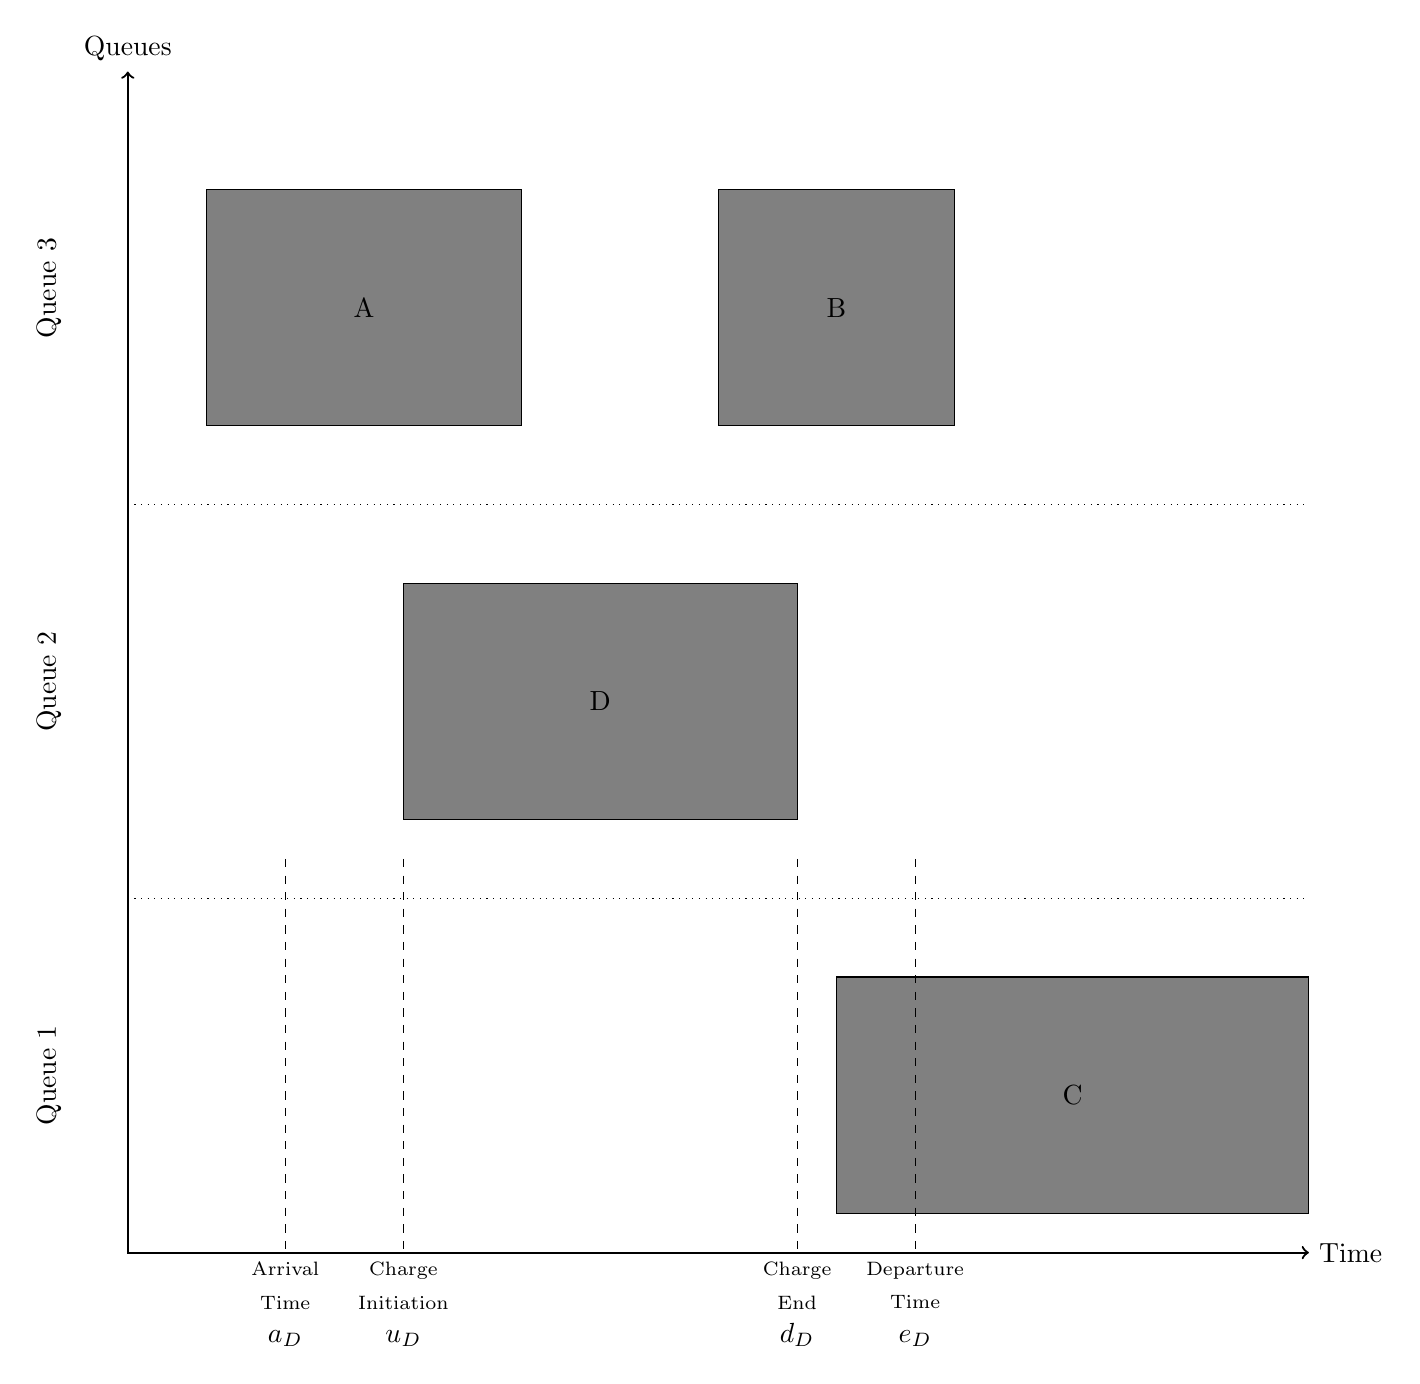
\begin{tikzpicture}
          % Variables
          \def \arrx   {2.0}
          \def \initx  {3.5}
          \def \endx   {8.5}
          \def \depx   {10.0}
          \def \yshift {5}

          % Axis
          \draw [thick,<->] (0,15) node[above]{Queues} -- (0,0) -- (15,0) node[right]{Time};

          % Rectangles
          \node[rectangle, draw, fill=gray, minimum width=4cm, minimum height = 3cm] at (3,12) {A};
          \node[rectangle, draw, fill=gray, minimum width=3cm, minimum height = 3cm] at (9,12) {B};
          \node[rectangle, draw, fill=gray, minimum width=5cm, minimum height = 3cm] at (6,7) {D};
          \node[rectangle, draw, fill=gray, minimum width=6cm, minimum height = 3cm] at (12,2) {C};

          % X-axis labels
          \node [below,align=center] at (\arrx,0) {\scriptsize Arrival     \\ \scriptsize Time \\ $a_D$};
          \node [below, align=center] at (\initx,0) {\scriptsize Charge    \\ \scriptsize Initiation  \\ $u_D$};
          \node [below, align=center] at (\endx,0) {\scriptsize Charge     \\ \scriptsize End \\ $d_D$};
          \node [below, align=center] at (\depx,0) {\scriptsize Departure  \\ \scriptsize Time \\ $e_D$};

          % Y-axis labels
          \node[rotate=90] at (-1, 2.25) {Queue 1};
          \node[rotate=90] at (-1, 7.25) {Queue 2};
          \node[rotate=90] at (-1, 12.25) {Queue 3};

          % Vertical lines
          \draw[dashed] (\arrx,\yshift)--(\arrx,0);
          \draw[dashed] (\initx,\yshift)--(\initx,0);
          \draw[dashed] (\endx,\yshift)--(\endx,0);
          \draw[dashed] (\depx,\yshift)--(\depx,0);

          % Horizontal lines
          \draw[dotted] (0, 4.5) -- (15, 4.5);
          \draw[dotted] (0, 9.5) -- (15, 9.5);

        \end{tikzpicture}
      }
      \caption{The representation of the queue-time space. The x and y-axis represent time and space, respectively. Along the y-axis, the dashed lines represent discrete queuing locations. The shaded rectangles represent schedules BEBs to be charged. The height of each shaded rectangle represents the space taken on the queue and the width being the time to service said BEB. The vertical dashed lines are associated with vessel D and represent the arrival time, initial charge time, charge completion time, and departure time. Note that the arrival time may be before the initial charge time and the completion time may before the departure time.}
      \label{fig:spacial-and-temporal-constr}
\end{figure}

\ref{seq:c0}-\ref{seq:c4} are denoted as ``queuing constraints''. They prevent overlap both spatially and temporally as
shown in \ref{fig:spacial-and-temporal-constr}. The y-axis represents the possible queues for a bus visit to be placed into, and the x-axis
represents the time that can be reserved for each visit. The shaded rectangles represent time that has been scheduled in
the horizontal direction, and the queue allocated for each bus visit in the vertical direction. In other words, the set
of constraints \ref{seq:c0} - \ref{seq:c4} aim to ensure that these shaded rectangles never overlap.

Constraint \ref{seq:c0} states that the starting charge time for BEB \(u_j\) must begin after the previous BEB departs,
\(d_i\). A value of \(\sigma_{ij} = 1 \implies\) bus \(i\) has detached from the charger before bus \(j\) has begun charging. If
\(\sigma_{ij} = 0\), then the constraint is of the form \(\T + d_i > u_j\) rendering the constraint ``inactive''. Similarly, for
\ref{seq:c1}, \(\psi_{ij}\) determines spacial positioning of BEB \(i\) and \(j\) relative to one another. A value of \(\psi_{ij} = 1
\implies\) BEB \(i\) is in a queue index that is less than BEB \(j\). If \(\psi_{ij} = 0\) then the constraint is deactivated.
Constraints \ref{seq:c2} - \ref{seq:c4} enforce spatial and temporal ordering between each queue/vehicle pair.
\ref{seq:c2} and \ref{seq:c3} ensure that BEB \(i\) is not placed before and after \(j\) spatially or temporally as that is
not possible. \ref{seq:c4} enforces at least one of the spatial or temporal relationships between each visit is active.
This ensures there are no scheduling conflicts (i.e. either charging sessions are ordered temporally or are in different
queues).

\ref{seq:c5} describes the service time of the bus. \ref{seq:c6} calculates the initial charge for the next visit for
bus \(b_i\). \ref{seq:c7} ensures that the bus is not being over-charged. \ref{seq:c8} ensures the continuity of the times
(i.e. the arrival time is less than the initial charge which is less than the detach time which is less than the time
the bus exits the station and all must be less than the time horizon).
\section{Simulated Annealing}
\label{sec:sa-simulated-annealing}
SA is a well-studied local search metaheuristic used to solve various optimization problems
\cite{gendreau-2018-handb-metah,press-1992-numer-recip}. The algorithm is often applied to problems that contain many
local solutions as it employs a stochastic approach that explores the solution space for an approximate global optimum.
This model is named after its analogized process where a crystalline solid is heated then allowed to cool at a slow rate
until it achieves its most regular possible crystal lattice configuration (i.e. lowest energy state)
\cite{henderson-1989-theor-pract,press-1992-numer-recip}. SA establishes a connection between the thermodynamic
process and the search for global optimum in optimization problems. Within the SA process there are three key components:
cooling schedule, acceptance criteria, and generation mechanisms
\cite{keller-2019-multi-objec,press-1992-numer-recip}.

The cooling equation describes the speed at which the figurative temperature is decreased in a controlled manner over
time. Throughout the SA process, many ``candidate'' solutions are generated and compared to an ``active'' solution. The
method by which the solutions are accepted is determined by the acceptance criteria. The acceptance criteria is a
function of the system temperature that makes the decision whether the system will accept an inferior solution in favor
of exploring the solution space. The means by which candidate solutions are generated is via the generation mechanisms.
These generators modify the solution by some singular discrete change \cite{gendreau-2018-handb-metah}. Each of these
components are elaborated in the subsequent sections.

\subsection{Cooling Equation}
\label{cooling-equation-experimental}
The cooling equation models the rate at which the temperature decreases over time in the SA process. Initially, when the
temperature is high, SA encourages exploration. As the process begins to ``cools down'' (in accordance to the cooling
schedule), it begins to encourage local exploitation of the solution (rather than exploration)
\cite{rutenbar-1989-simul-anneal-algor,henderson-1989-theor-pract}. There are three common basic types of cooling
equations: linear, geometric, and exponential. Geometric cooling schedules are most widely used in practice
\cite{keller-2019-multi-objec}. As such, it will also be employed by this work. It is defined by the difference
equation

\begin{equation}
\label{eq:cool}
t_m = \beta t_{m-1}\text{.}
\end{equation}

In \ref{eq:cool}, \(\beta\) controls the cooling rate. Typical values of \(\beta\) are within the range \([0.8, 0.99]\)
\cite{henderson-1989-theor-pract}. \ref{fig:geometric} demonstrates this principle by plotting the geometric schedule
using varying values of \(\beta\). The variable \(t_m\) represents the temperature at the \(m^{\text{th}}\) step of the temperature
function. The total amount of steps \(M\) is dictated by the initial temperature and \(\beta\).

\begin{figure}[t!]
  \centering 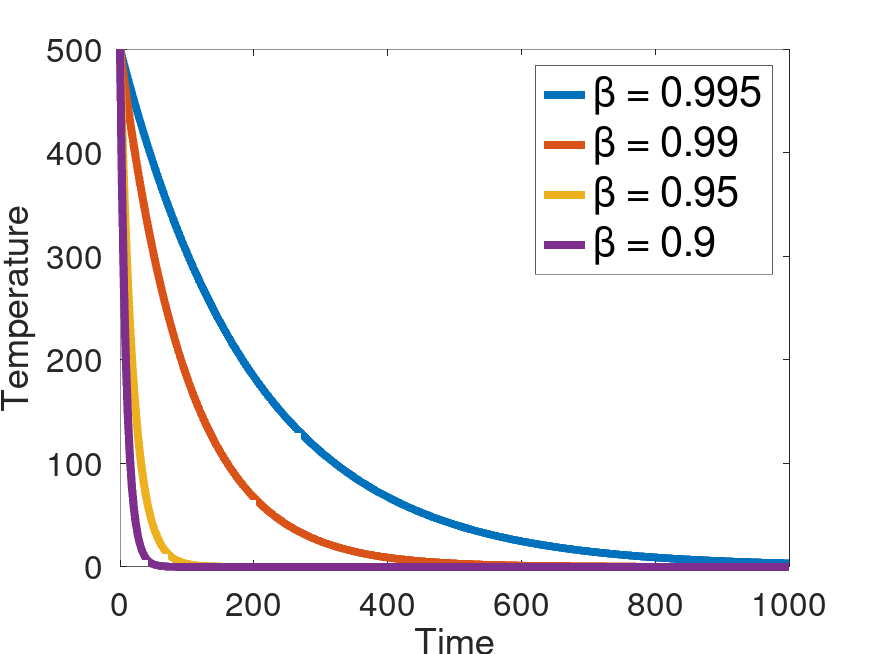
\includegraphics[width=0.6\textwidth]{img/geometric.png}
  \caption{Geometric cooling schedule utilizing various value of $\beta$.}
  \label{fig:geometric}
\end{figure}

\subsection{Acceptance Criteria}
\label{sec:sa-acceptance}
In SA, the algorithm stores a solution that is continuously compared to newly generated solutions. Let the stored
solution be referred to as the ``active solution''. During each iteration, a new ``candidate'' solution is generated and
compared to the active solution to determine if the candidate solution should replace the active solution. The method of
determining whether the active solution should be replaced is defined by an acceptance criteria. In an effort to
encourage exploration, inferior candidate solutions have a probability of being accepted. The probability of accepting
an inferior candidate solution is determined by the objective functions of the active and candidate solutions, \(J(\I)\)
and \(J(\bar{\I})\), respectively, and the current temperature, \(t_m\). Let \(\Delta E \equiv J(\I) - J(\bar{\I})\) and let \(f(\cdot)\) be
the function that describes the probability of accepting a candidate solution \(\bar{\I}\). The probability of accepting a
candidate solution is thus of the form \cite{keller-2019-multi-objec}

\begin{equation}
\label{eq:candaccept}
f(\I,\bar{\I},t_m) =
\begin{cases}
  1                   & \Delta E > 0 \\
  e^{- \frac{\Delta E}{t_m}} & \text{otherwise}
\end{cases}\text{.}
\end{equation}

\subsection{Neighbor Generators and Wrappers}
\label{sec:sa-generation-mechanisms}
Generation mechanisms are used to create a neighboring candidate solution \cite{gendreau-2018-handb-metah}. That is,
the generating function creates a solution that can be reached in a single iteration from the active solution. In
response to the problem statement made in \ref{sec:sa-problem-description}, five primitive generation mechanism are used: new
visit, slide visit, new charger, new window, wait. The purpose of each of these generators is to assign new visits to a
charger, adjust a bus visits initial and final charge time within the same time frame/queue, move a BEB from one charger
to another with the same charge schedule, move a bus to its idle queue. Each generator will be discussed in more detail
in \ref{sec:sa-generators}.

These primitive generation mechanisms will, in turn, be utilized by two wrapper functions. The charge schedule generator
is to used create an initial candidate solutions for SA and the perturb schedule generator is used to take a candidate
solution and alter it slightly in an attempt to step toward a global or local minimum. The wrapper functions will be
discussed in \ref{sec:sa-generator-wrappers}. However, prior to discussing the primitives and wrapper generating functions,
their respective inputs and outputs must be defined.

\subsubsection{Generator Input/Output}
\label{sec:sa-generator-input-output}
Each generator accepts a tuple \(\Sol \equiv (i, \I, \C)\) where \(i\) is the visit index being manipulated, \(\I\) is the set of
visits, and \(\C\) is the set that describes the availability for all chargers \(q \in \Qset\). The output of the generating
functions is the same as the input, but with changes applied to it by a generator. Let a modified variable be denoted
with a bar, \(\bar{\cdot}\). Thus, the modified input tuple is written as \(\bar{\Sol}\).

\subsubsection{Generators}
\label{sec:sa-generators}
The mechanism by which candidate solutions are generated is introduced in the subsequent sections. Recall that to
satisfy constraints, \(n_B\) extra idle queues are added that provide no power to the BEB. Because of this, the set of
queues is fully defined where \(Q\) is the ordered set of idle queues, slow queues, then fast queue. The use case for the
idle queues are for when a bus is not to be placed on a charger. Rather, it will be placed in the queue, \(q \in B\), which
satisfies the previously defined spatial constraints while allowing the bus to be ``set aside''. The charge queues are
denoted by \(q \in \{1, ..., n_B , n_B + 1, ..., n_Q\}\).

For the sake of ease in referring to the various variables associated with a visit, dot notation is used. For example,
suppose the arrival time is desired to be extracted from visit \(i\). Given \(\I\), the notation that describes extracting
the initial charge time for visit \(i\) is written as \(u_i \equiv \I_{i.u}\).

\paragraph{New visit}
\label{sec:sa-new-visit}
The new visit generator defined in \ref{alg:new-visit} describes the process of moving a BEB, \(b \in B\), from a waiting
queue, \(q \in B\), to a charging queue, \(q_i \in \{n_B + 1, ..., n_Q\}\), within its arrival/departure time \([a_i, e_i]\). Let
\(\U_{\{\cdot\}}\) indicate that an element is selected randomly with a uniform distribution from the set \(\{\cdot\}\). For
example, \(\U_{[a_i, e_i]}\) indicates that a value will be selected between \(a\) and \(e\) with a uniform distribution.
\ref{alg:new-visit} begins by extracting variables. Lines 6 and 7 randomly select a charging queue and available time
frame with a uniform distribution, respectively. Line 8 attempts to assign the visit the time frame found in Line 7, if
it succeeds, the updated visit is returned. Otherwise, the null value is returned.

The function \texttt{findFreeTime} is the algorithm that determines whether a visit's time at the station \([a_i, e_i]\) can be placed
in the time availability of charger \(q\). Let the available time for charger \(q\) for visit \(i\) be denoted as \(C \equiv
\C_{i.q}\). Furthermore, let the lower and upper bound of \(\C\) be denoted as \(C_L\) and \(C_U\), respectively. The algorithm
checks whether the BEB time at the station, \([a_i, e_i]\) fits within the charger availability \([C_L, C_U]\). If it does,
a random charging time frame is returned such that \(a_i \le u_i \le d_i \le e_i\). Otherwise the null value is returned.

\begin{algorithm}[H]
  \scriptsize
  \caption{New visit algorithm}
  \label{alg:new-visit}
  \LinesNumbered
  \TitleOfAlgo{New Visit}
  \KwIn{$\Sol$}
  \KwOut{$\bar{\Sol}$}

  \SetKwFunction{Union}{Union}
  \SetKwFunction{FindFreeTime}{FindFreeTime}

  \Begin
    {
      $i \leftarrow \Sol_{i}$\tcc*{Extract visit index}
      $a \leftarrow \I_{i.a}$\tcc*{Extract the arrivial time for visit $i$}
      $e \leftarrow \I_{i.e}$\tcc*{Extract the departure time for visit $i$}
      $q \leftarrow \I_{i.q}$\tcc*{Extract the current charge queue for visit $i$}
      $\bar{q} \leftarrow \mathcal{U}_{Q}$\tcc*{Select a random charging queue with a uniform distribution}
      $C \leftarrow \mathcal{U}_{\C_q}$\tcc*{Select a random time slice from $\C_q$}

      \If(\tcc*[f]{If there is time available in $C_q^j$}){($\bar{C}, \bar{u}, \bar{d}$) $\leftarrow$ \FindFreeTime{$C, i, q, a, e$} $\not\in \varnothing$}
         {
           \Return{($i, (\bar{q},\bar{u},\bar{d}),\bar{C}$)}\tcc*[f]{Return visit}
         }

         \Return{($\varnothing$)}\tcc*{Return nothing}
    }
\end{algorithm}

\paragraph{Slide visit}
\label{slide-visit}
This primitive generator is used for visits that have already been scheduled. Because of the constraint \ref{seq:c8},
there may be some slack to manipulate \([u_i, d_i]\) within the window \([a_i, e_i]\). That is, two new values, \(u_i\) and
\(d_i\) are randomly selected with a uniform distribution that satisfy the constraint \(a_i \leq u_i \leq d_i \leq e_i\). Line 2 of
\ref{alg:slide-visit} purges the visit from the charger availability schedule. The \texttt{Purge} function simply removes an
assigned charge time from the set \(\C\). Without altering selected queue, the charge time randomly re-assigned with a
uniform distribution. Upon success, the updated tuple is returned, otherwise the null value is returned.

\begin{algorithm}[H]
  \scriptsize
  \caption{Slide Visit Algorithm} \label{alg:slide-visit}
  \LinesNumbered
  \TitleOfAlgo{Slide Visit}
  \KwIn{$\Sol$}
  \KwOut{$\bar{\Sol}$}

    \SetKwFunction{Purge}{Purge}

    \Begin
    {
      $(i, \I, \bar{\C}) \leftarrow$\Purge{$\Sol$}\tcc*{Purge visit $i$ from charger availibility matrix}
      $C \leftarrow \bar{C}_{i.q_i}$\tcc*{Get the time availability of the purged visit}

      \tcc{If there is time available in $C$}
      \If{($\bar{C}, \bar{u}, \bar{d}$) $\leftarrow$ \FindFreeTime{$C$, $\Sol_i$, $\I_q$, $\I_{i.a}, \I_{i.e}$} $\not\in \varnothing$}
      {
        \Return{($i, \I, (\I_{i.q_i},\bar{u},\bar{d}),\bar{C}$)}\tcc*[f]{Return updated visit}
      }

        \Return{($\varnothing$)}\tcc*{Return nothing}
    }
  \end{algorithm}

\paragraph{New charger}
\label{new-charger}
The new charger generator moves a visit \(\I_i\) to a new charging queue while maintaining the same charge time, \([u_i,
d_i]\). \ref{alg:new-charger} purges the visit from the charger availability set, a queue is selected at random with a
uniform distribution, then the new selection is checked whether the charge time \([u_i, d_i]\) may be assigned to the new
queue.

\begin{algorithm}[H]
  \scriptsize
  \caption{New Charger Algorithm} \label{alg:new-charger} \LinesNumbered \TitleOfAlgo{New Charger} \KwIn{$\Sol$}
  \KwOut{$\bar{\Sol}$}

    \SetKwFunction{Purge}{Purge}

    \Begin
    {
      $(i, \I, \bar{\C}) \leftarrow$\Purge{$\Sol$}\tcc*{Purge visit $i$ from charger availibility matrix}
      $q \leftarrow \mathcal{U}_{Q}$\tcc*{Select a random charging queue with a uniform distribution}

      \If(\tcc*[f]{If there is time available in $C_{q}$}){($\bar{C}, \bar{u}, \bar{d}$) $\leftarrow$ \FindFreeTime{$\bar{\C}_{i.q}$, $\Sol_i$, $\I_q$, $\I_{i.a}, \I_{i.e}$} $\not\in \varnothing$}
      {
        \tcc{Return visit, note $u$ and $d$ are the original inital/final charge times.}
        \Return{($i, \I, (q,\I_{i.u}, \I_{i.d}),\bar{\C}$)}
      }

      \Return{($\varnothing$)}\tcc*{Return nothing}
    }
  \end{algorithm}

\paragraph{Wait}
\label{sec:sa-wait}
The wait generator simply removes a bus from a charger queue and places it in its idle queue, \(q_i \in B\). \ref{alg:wait}
begins by purging the visit from the charger availability set, the visit is then assigned to its idle queue for the
duration of its time at the station.

\begin{algorithm}[H]
\scriptsize
\caption{Wait algorithm} \label{alg:wait}
    \LinesNumbered
    \TitleOfAlgo{Wait}
    \KwIn{$\Sol$}
    \KwOut{$\bar{\Sol}$}

    \SetKwFunction{Purge}{Purge}

    \Begin
    {
      $(i, \I, \bar{\C}) \leftarrow$\Purge{$\Sol$}\tcc*{Purge visit $i$ from charger availibility matrix}
      \tcc{Update the charger availability matrix for wait queue $\bar{\C}_{i.q_i}$}
      $\bar{\C}'_{\I_{i.\Gamma_i}} \leftarrow \C' \cup \{[\I_{i.a}, \I_{i.e}]\}$\;
      \Return{$(i, \I, (\I_{i.b}, \I_{i.a}, \I_{i.e}), \bar{\C})$}\tcc*[f]{Return visit}
    }
  \end{algorithm}

\paragraph{New Window}
\label{sec:sa-new-window}
New window, as shown in \ref{alg:new-window}, is a combination of \ref{alg:new-visit} (new visit) and \ref{alg:wait}
(wait). By this it is meant that visit \(i\) is placed in its wait queue then added back in as if it were a new visit.
This implies that the BEB may be assigned to a different queue with a new charging time frame. Upon success, the
algorithm return the updated tuple, otherwise return the null value.

\begin{algorithm}[H]
  \scriptsize
  \caption{New window algorithm} \label{alg:new-window}
  \LinesNumbered
  \TitleOfAlgo{New Window}
  \KwIn{$\Sol$}
  \KwOut{$\bar{\Sol}$}

  \SetKwFunction{NewVisit}{NewVisit}
  \SetKwFunction{Wait}{Wait}

  \Begin
  {
    $\bar{\Sol} \leftarrow$\Wait{$\Sol$}\tcc*{Assign visit to its respective idle queue}
    \If(\tcc*[f]{Add visit $i$ back in randomly})
       {
         $\bar{\bar{\Sol}} \leftarrow$ \NewVisit{$\bar{\Sol}$} $\not\in \varnothing$
       }
       {
         \Return{$\bar{\bar{\Sol}}$} \tcc*[f]{Return visit}
       }

       \Return{($\varnothing$)}\tcc*{Return nothing}
  }
\end{algorithm}

\subsubsection{Generator Wrappers}
\label{sec:sa-generator-wrappers}
The generator wrappers provide the highest level of abstraction from which the SA algorithm directly interacts. These
wrapper functions utilize the primitive generators previously described to either create a new charge schedule to
initialize the SA algorithm, or to modify an existing schedule.

\paragraph{Charge Schedule Generation}
\label{sec:sa-charge-schedule-generation}
The objective of \ref{alg:charge-schedule-generation} is introduce a method that provides the SA algorithm with an
initial charging schedule. The schedule generation is chosen to initialize the algorithm in a greedy manner by looping
through each visit and executing \ref{alg:new-visit} to place visit \(i\) at random queue with a random charge time.

\begin{algorithm}[H]
\scriptsize
\caption{Charge schedule generation algorithm} \label{alg:charge-schedule-generation}
    \LinesNumbered
    \TitleOfAlgo{Candidate Solution Generator}
    \KwIn{$(\I, \C)$}
    \KwOut{$(\bar{\I}, \bar{\C})$}

    \SetKwFunction{NewVisit}{NewVisit}

    \Begin
    {
        \tcc{Select an unscheduled BEB visit from a randomly indexed set of visits}
        \ForEach {$\I_i \in \I$}
        {
            ($i, \bar{\I}$, $\bar{\C}$) $\leftarrow$ \NewVisit{($\I_i$, $\I$, $\C$)}\tcc*{Assign the bus to a charger}
        }
            \Return{($\bar{\I}$, $\bar{\C}$)}
    }
  \end{algorithm}

\paragraph{Perturb Schedule}
\label{sec:sa-tweak-schedule}
\ref{alg:perturb-schedule} describes the method by which the SA algorithm decides how to perturb a given charge
schedule. The method that will be employed to generate neighboring solutions is as follows: pick a visit, pick a
primitive generator, and execute said primitive generator once. Let \(\W^y_{[\cdot]}\) denote a random selection with a
distribution specified by a weight vector \(y \in \mathbb{R}\). Thus, \ref{alg:perturb-schedule} is as follows: Lines 2-12 generate a
vector of weights for the visit index selection. The weights have a default value of one. Each visit is then indexed in
reverse order. If the SOC of the visit is less than \(\nu_b \kappa_b\), then the weight for the visit is calculated as shown on
Line 10. The route for BEB \(b\) is then set as a ``priority'' on Line 9 to propagate the previously calculated weight in
earlier visits for BEB \(b\) as shown on Line 5. This is done in an attempt to encourage the SA algorithm to ``fix'' the
current or previous visits so that the SOC stays above the minimum threshold. The algorithm then selects a visit index
with weighted distribution \(y^v\), then selects a primitive with a weighted distribution, \(y^p\). Letting \(n_G\) denote the
number of primitive generating functions, the selected primitive with a weighted distribution is denoted as
\(\W^{y^v}_{[1, n_G]}\). The primitive is then executed, and the results are returned.

\begin{algorithm}[H]
\scriptsize
\caption{Perturb schedule algorithm} \label{alg:perturb-schedule}

    \LinesNumbered
    \TitleOfAlgo{Perturb Schedule}
    \KwIn{$(\I, \C)$}
    \KwOut{$(\bar{\I}, \bar{\C})$}

    \SetKwFunction{PrimitiveGeneratingFunction}{PrimitiveGeneratingFunction}

    \Begin
    {
        $p \leftarrow [false; n_A]$\tcc*{Create vector to track priority routes}
        $y^v \leftarrow [1.0; n_V]$\tcc*{Create weight vector for index selection}
        \tcc{Loop through the visits in reverse order}
        \ForEach{$\I_i \leftarrow \I_{|\I|} \text{ TO } \I_{1}$}
        {
            \tcc{If the current visit is part of a priority route}
            \If{$p_{\I_{i.b}} = true$}{$y^v_{\I_i} = y^v_{\I_{i.\xi}}$\;}
            \tcc{Else if the current visit's SOC does below the allowed threshold}
            \ElseIf{$\I_{i.\eta} \le \nu_{\I_{i.b}} \kappa_{\I_{i.b}}$}{
                $p_{\I_{i.b}} = true$\tcc*{Indicate the current BEB's routes are to be prioritized}
                $y^v_{\I_i} = \kappa_{\I_{i.b}} + \kappa_{\I_{i.b}} (\nu_{\I_{i.b}}\kappa_{\I_{i.b}} - \I_{i.\eta})$\tcc*{Calculate the weight of the current visit}
            }
        }
        $\I_i\leftarrow\; \W^{y^v}_{\I}$\tcc*{Select an index with a weighted distribution}
        $y^p \leftarrow [y^p_1, y^p_2, ...]$\tcc*{Define the weight of each primitive generator}
        \tcc{Select a generator function with weighted distribution}
        $PrimitiveGeneratingFunction \leftarrow\; \W^{y^p}_{[1,n_G]}$\;
        $\bar{\Sol} \leftarrow$ \PrimitiveGeneratingFunction{($\I_i$, $\I$, $\C$)}\tcc*{Excecute the generator function}
        \Return{($\bar{\I}$, $\bar{\C}$)}
    }
\end{algorithm}

\subsection{Alternative Heuristic Implementation}
\label{sec:sa-heuristic-implementation}
As suggested by the works in \cite{Zhang_2010,Xinchao_2011}, applying heuristics to the generating functions can
manipulate the searched neighborhoods in a way that may assist the SA algorithm with convergence. As a test to assist in
minimizing charger utilization, a simple heuristic is applied to \ref{alg:new-visit} and \ref{alg:new-charger} in the
method that they select new charging queues. Rather than selecting a queue at random from \(q \in Q\), the algorithms
randomly select whether to place a BEB in a slow or fast charging queue with a weighted distribution favoring slow
chargers. Once the charger type has been selected, the algorithm will then begin incrementally attempting to place the
BEB in a queue of that type beginning from the smallest index of that charger type. For example, if a BEB has been
selected to be placed in a queue with a slow charger, the algorithm begins by attempting to place the BEB in the charger
queue \(q = n_B + 1\). If it is unable to be placed in that queue, it then attempts to be placed in the next queue \(q =
n_B + 2\). This is done incrementally until all the queues have been exhausted. The objective of this alternative
approach is to explore whether the added up-front computation cost by including the heuristic will positively influence
the output of the results and to what degree.
\section{Optimization Algorithm}
\label{sec:sa-optimization-algorithm}
This section combines the generation algorithms and the optimization problem into a single algorithm (\ref{alg:sa-pap}).
Generally, SA assumes that the generated candidate solutions are within the solution space of the problem, \(\omega \in S\) where
\(S\) is the solution space. Hence, the initialization and perturbations of a schedule must be verified to ensure that the
generated schedule is in the solution space. Therefore, the objective function and constraints introduced in
\ref{sec:sa-constraints} and \ref{sec:sa-objective-function}, respectively, must be employed to verify that the outputs of
\ref{alg:charge-schedule-generation} and \ref{alg:perturb-schedule} are in the feasible space, \(S\).

As previously stated, the generating functions directly influence the values of the assigned charge queue, charge
initialization time, and charge completion time: \(q_i\), \(u_i\), and \(d_i\), respectively. Having generated those values,
the rest of the decision variables may be derived. Beginning with the packing constraints, \ref{seq:c0}-\ref{seq:c1} are
employed to enable and disable \(\sigma_{ij}\) and \(\psi_{ij}\) and \ref{seq:c2}-\ref{seq:c4} ensure the validity of the values.
\ref{seq:c5} can be directly calculated and \ref{seq:c8} is fully defined.

Changing the focus over to the dynamic constraints, similarly to what was seen with the packing constraints, the battery
dynamic constraints are also fully defined. \ref{seq:c6} is sequentially calculated after a given schedule has been
fully defined. \ref{seq:c7} is evaluated to ensure the BEB is not overcharged. The penalty method implemented in
\ref{sec:sa-objective-function} is set in place to allow the SOC to go below the specified threshold, \(\nu_{b_i} \kappa_{b_i}\), but
punish the solution for doing so. Thus, over time, the candidate solutions will be encouraged toward a solution that
does not activate the penalty method (i.e., is solution is operationally feasible).

The implementation of the SA PAP is outlined in \ref{alg:sa-pap} will now be outlined. The algorithm begins by creating
a temperature schedule and creating an initial solution. The algorithm then iterates through the temperature schedule
(outer loop). For each iteration of the outer loop, an inner loop is executed \(n_K\) times. During this inner loop, the
solution is modified by a primitive generating function to create a candidate solution. The candidate is solution is
then compared with the active solution, and updated according to the acceptance criteria. These actions are performed
until the cooling equation is exhausted.

\begin{algorithm}[H]
  \scriptsize
  \caption{Simulated annealing approach to the position allocation problem} \label{alg:sa-pap}
  \LinesNumbered
  \TitleOfAlgo{SA PAP}
  \KwIn{($\I$ , $\C$)}
  \KwOut{($\bar{\I}$, $\bar{\C}$)}

  \SetKwFunction{Temp}{$\Tau$}
  \SetKwFunction{ChargeScheduleGenerator}{ChargeScheduleGenerator}
  \SetKwFunction{PerturbSchedule}{PerturbSchedule}
  \SetKwFunction{Obj}{J}

  \Begin
    {
      \tcc{Generate vector of temperatures given cooling equation $\Tau$ and initial temperature $\Tau_0$}
      $t \leftarrow$ \Temp{$\Tau_0$}

      $\Sol \leftarrow$\ChargeScheduleGenerator{($\I$, $\C$)}\tcc{Generate an initial solution}

      \tcc{For each item in the temperature vector}
      \ForEach{$t_k \in t$}
       {
        \tcc{For each step in the constant temperature repitition counter}
        \ForEach{$k \in \{0, 1, ..., n_K\}$}
        {
          $\bar{\Sol} \leftarrow$ \PerturbSchedule{($\I$, $\C$)} \tcc*{Generate a new solution}
          $\Delta E = $ \Obj{$\bar{\Sol}_{\I}$}  - \Obj{$\Sol_{\I}$} \tcc*{Calculate the difference of fitness scores}

          \If{$\bar{\I} \in S$ and $\Delta E < 0$}{$\Sol \leftarrow \bar{\Sol}$}
          \If{$\bar{\I} \in S$ and $\Delta E \ge 0$}{$\Sol \leftarrow \bar{\Sol}$ with probability $e^{\frac{\Delta E}{t_k}}$}
        } % For k
      }   % For t_k \in t

      \Return{($\I$ , $\bar{\C}$)}
    } % Begin
\end{algorithm}

\section{Example}
\label{sec:sa-example}
An example is now provided to demonstrate the utility of the developed SA charge scheduling technique. In
\ref{sec:sa-beb-scenario} a description of the example scenario is presented followed by a brief introduction of the BEB
implementation of the BPAP. An alternative threshold based planning strategy called the Qin-Modified technique, and a
heuristic modification to the SA PAP are also used as comparisons to the SA PAP technique presented in this work.
\ref{sec:sa-results} presents the results for each of planning strategies. The results are then analyzed and discussed.

\subsection{BEB Scenario}
\label{sec:sa-beb-scenario}
The test scenario was run over a time horizon of \(T=24\) hours, with a total of \(n_V = \N\) visits to the station shared
between \(n_B = \A\) buses. Each BEB is assumed to have a battery capacity of \(\kappa_b =\) \batsize kWh that is required to
stay above an SOC of \(\nu_b =\) \mincharge (\num{\fpeval{\batsize * \minchargeD}} kWh). Each bus is assumed to
begin the working day with \(\alpha =\) \num{\fpeval{\acharge*100}}\% charge (\num{\fpeval{\acharge * \batsize}} kWh). A total of \num{\fpeval{\fast + \slow}} chargers are utilized where \slow of the chargers
are slow charging (\slows kW) and \fast are fast charging (\fasts kW). The gains of \(z_p\) \num{\Cgain}, \(z_c
= 1\), and \(z_d =\) \num{10000} are used. As previously introduced, to encourage the SA PAP to utilize the
fewest number of chargers, the value of \(\epsilon_q\) in the objective function is \(\forall q \in \{1,2,..., n_B \}; \epsilon_q = 0\) and \(\forall q \in
\{n_B + 1, n_B + 2, ..., n_Q\}; \epsilon_q = 10q\). The SA algorithm utilizes the geometric cooling schedule with an initial
temperature of \(T_0 =\) \num{\tempinit} with \(\beta = 0.997\), resulting in a total of \(n_M =\)
\num{\tempcnt} steps. Rocky Mountain Power utilizes fifteen-minute intervals to calculate the demand cost
\cite{rocky-mountain-power}. To estimate the method by which Rocky Mountain Power determines its demand cost, this work
employed an interval of \(T_p =\) \num{\fpeval{15*60}} seconds in its demand cost calculation. A weight vector
of \([0.6255, 0.6255, 0.4170, 0.2085]\) is used to influence the distribution of selecting the new charger, new window,
wait, and slide visit primitives, respectively. The algorithm also assumes a total of \(n_K = \localcnt\) iterations for
the local search at a constant temperature. In total, that results in \num{\fpeval{\localcnt * \tempcnt}}
configurations being searched in a total runtime of \num{\fpeval{\quicklocal * \tempcnt}} seconds.

\ref{sec:sa-heuristic-implementation} introduced the idea of an alternative heuristic implementation for the SA algorithm. To
distinguish the heuristic implementation from the method derived in \ref{sec:sa-generation-mechanisms}, let this
implementation be referred to as ``heuristic'' implementation and the previous as the ``quick'' implementation due to the
fact that it is designed to execute more quickly. Using the same weights for randomly selecting the primitive
generators, the heuristic approach further implemented a weighted distribution vector of \([0.9487, 0.3162]\) to decide
whether to select a slow or fast charger, respectively. The heuristic approach had a total runtime of
\num{\fpeval{\heuristiclocal * \tempcnt}} seconds. The heuristic generators were expected to be slightly
slower due to its iterative approach.

The Qin-Modified is a threshold-based strategy that is also employed as a means of comparison with the results of the SA
BPAP. The Qin-Modified algorithm is a based on the threshold strategy of \cite{qin-2016-numer-analy}. The algorithm has
been modified slightly to accommodate the case of multiple charger types without a heuristic search for the best charger
type. The heuristic is based on a set of rules that revolve around the initial charge of the bus at visit \(i\). There are
three different thresholds, low (40\%), medium (70\%), and high (90\%). Buses below the low threshold are prioritized to
fast chargers then are allowed to utilize slow chargers if no fast chargers are available. Buses between the low and
medium threshold prioritize slow chargers first and utilize fast chargers only if no slow chargers are available. Buses
above the medium threshold and below high will only be assigned to slow chargers. Buses above the high threshold will
not be charged. Once a bus has been assigned to a charger, it remains on the charger for the duration of the time it is
at the station, or it reaches 90\% charge, whichever comes first.

Another method utilized to compare with against SA PAP is the BEB implementation of the BPAP. The BPAP implementation is
utilized in this work as a benchmark for the other schedules as it is implemented utilizing a commercial solver. The
inputs to the system are the same as those discussed above. It is of note that the BPAP does not implement the demand
cost in its objective function. In an attempt to compare the solution of the BPAP with the SA output more directly, a
similar solve time of 1,900 seconds is utilized. The BPAP was executed using the Gurobi MILP solver
\cite{gurobi-2021-gurob-optim}. The previously described simulations were run on a machine equipped with an AMD Ryzen 9
5900X 12 - Processor (24 core) at 4.95GHz.

\subsection{Results}
\label{sec:sa-results}
The schedules generated by each of the methods is presented in \ref{fig:schedule}. For the sake of conciseness of the
schedule plots, the waiting queues are excluded. Therefore, rows 0-14 represent slow charging queues and rows 15-29
represent fast charging queues. The hollow circles with an 'X' represent the initial charge times, and the horizontal
line with the vertical tick signifies the region of time the charger is active. The Qin-Modified schedule utilized two
fast and chargers and fourteen slow chargers as can be seen in \ref{subfig:schedule-qin}. The BPAP framework generated a
schedule that utilizes three fast charges and four slow chargers as shown in \ref{subfig:schedule-milp}. The heuristic
SA strategy created a schedule with nine slow charger queues and one fast charging queue as shown in
\ref{subfig:schedule-heuristic-sa}. The quick strategy for the SA algorithm created a schedule utilizing seven slow
chargers and two fast chargers as is demonstrated in \ref{subfig:schedule-quick-sa}. That is to say, while each schedule
emphasized the utilization of slow chargers, the Qin-Modified required fast charging most frequently followed by the
BPAP, quick SA, and then heuristic SA. At the expense of incorporating more slow chargers than the BPAP, the SA
techniques chose to utilize fast chargers less frequently in their respective schedules showing an emphasis on battery
health.

\ref{tab:charge} tabulates the mean, minimum, and maximum SOC upon arrival for each visit. The BPAP requires each BEB to stay
above an SOC of 25\% while the quick and heuristic SA approaches heavily penalize a schedule for allowing a BEB to go
below the 25\% SOC threshold. The BPAP was able to successfully keep the SOC above the threshold while both SA approaches
were a few kWh below the threshold. The SOC of the quick SA approach dropped to a minimum of 96.996 kWh and the
heuristic had a minimum SOC of 96.270 kWh as shown in \ref{tab:charge}. Due to the threshold constraint being soft, the SA
objective function may find it bettor to allow a small deficit in the threshold penalty function in favor of another
action. As a remedy to ensure the SA schedules stay above the threshold, a safety factor could be introduced to
artificially increase the threshold, \(S_f \nu_{b_i}\kappa_{b_i}\) where \(S_f > 1;\; S_f \in \mathbb{R}\). The Qin-Modified schedule allowed
the SOC for one of the BEBs to reach 0\% as shown in \ref{tab:charge}. The Qin-Modified strategy, being a purely reactive
model, does not have foresight to determine whether a set of routes has a particularly taxing route later in the time
horizon. As such, and in the case of the example scenario, the BEB that reached a charge of 0\% began with a sequence of
short routes, much like the other BEBs. However, rather than continuing this trend, these sets of routes had one or two
longer routes which the Qin-Modified algorithm was unable to account for. Interestingly, Qin-Modified strategy was able
to keep the mean SOC the highest followed by the quick SA, heuristic SA, and then the BPAP.

\begin{table}[htbp]
\caption{\label{tab:charge}Table of mean, min, and max SOC (kWh) for each charging schedule.}
\centering
\begin{tabular}{l|cccc}
\hline
 & BPAP & Qin-Modifid & Heuristic & Quick\\[0pt]
\hline
Mean & 181.327 & 275.045 & 185.443 & 191.937\\[0pt]
Min & 97.000 & 0.000 & 96.270 & 96.996\\[0pt]
Max & 382.93 & 380.840 & 388.907 & 388.000\\[0pt]
\hline
\end{tabular}
\end{table}

\ref{fig:power} depicts the power utilized over the time horizon for each model. As previous stated, the Qin-Modified
schedule had the highest mean SOC over the working day. Referencing \ref{fig:power-usage-milp-qin}, the Qin maintained
long periods of steady slow and fast charger use. This is again a symptom of the Qin-Modified strategy placing BEBs on
chargers solely based on the SOC upon arrival. The BPAP and SA techniques, while having peaks in the first half of the
time horizon, were able to effectively maintain lower demand profiles during slower moments throughout the day.
\ref{fig:power} is also of interest as it shows the peak power demand over the time horizon. The peaks for each schedule
shown in \ref{tab:power}. While the quick SA was unable to beat the BPAP in peak demand (61 kW difference), the
heuristic SA was able to keep the peak power demand at 1180 kW (730 kW difference).

\begin{table}[htbp]
\caption{\label{tab:power}Table of mean and max power demand for each charging schedule.}
\centering
\begin{tabular}{l|cccc}
\hline
 & BPAP & Qin-Modified & Heuristic & Quick\\[0pt]
\hline
Mean & 176.550 & 394.13 & 181.583 & 186.858\\[0pt]
Max & 1910.000 & 2000 & 1180.950 & 1981.8999\\[0pt]
\hline
\end{tabular}
\end{table}

The total energy consumed by each schedule is shown in \ref{fig:energy-usage}. The ordering of most energy consumed to
least is as follows: Qin-Modified, heuristic SA, quick SA, and the BPAP. The respective energy consumption for each
technique is: 9,459.120 kWh, 4,357.609 kWh, 4,340.609 kWh, and 4,237.200 kWh. The quick SA consuming about 103 kWh more
than the BPAP. While the quick and heuristic SA were unable to match the BPAP in energy consumption, it is a trade-off
made by increasing the number of slow chargers and charge duration, and reducing the peak demand.

\begin{table}[htbp]
\caption{\label{tab:scores}Table of objective function scores for each of the schedules.}
\centering
\begin{tabular}{l|c}
\hline
Schedule & Score\\[0pt]
\hline
BPAP & \num{185000000}\\[0pt]
Qin-Modified & \num{190886308}\\[0pt]
Heuristic & \num{171367626}\\[0pt]
Quick & \num{180175082}\\[0pt]
\hline
\end{tabular}
\end{table}

As a final comparison, the scores for the Qin-Modified, quick SA, BPAP, and heuristic SA as shown in \ref{tab:scores}. The
Qin-Modified strategy naturally has the highest score as it performed the worst in each component of the objective
function. The BPAP beat the quick SA technique due to the consumption and demand costs. The heuristic SA was able to
successfully obtain the lowest score due to its substantial reduction in the demand cost. This shows that the added
queue selection bias toward slow chargers assisted the heuristic SA to converge more quickly. The quick SA technique, on
the other hand, had a slower rate of convergence due to its random queue placement.

\begin{figure}
  \centering
  %~~~~~~~~~~~~~~~~~~~~~~~~~~~~~~~~~~~~~~~~~~~~~~~~~~~~~~~~~~~~~~~~~~~~~~~~~~~~
  % Qin
  \begin{subfigure}[t]{\textwidth}
    \centering
    \includegraphics[width=\textwidth]{img/schedule-quinn}
    \mysubcaption{Charging schedule generated by Qin Modified algorithm.}
    \label{subfig:schedule-qin}
  \end{subfigure}

  \hfill

  %%~~~~~~~~~~~~~~~~~~~~~~~~~~~~~~~~~~~~~~~~~~~~~~~~~~~~~~~~~~~~~~~~~~~~~~~~~~~~
  % BPAP
  \begin{subfigure}[t]{\textwidth}
    \centering
    \includegraphics[width=\textwidth]{img/schedule-milp}
    \mysubcaption{Charging schedule generating by the BPAP algorithm.}
    \label{subfig:schedule-milp}
  \end{subfigure}
\end{figure}

\begin{figure} \ContinuedFloat
  \centering

  %%~~~~~~~~~~~~~~~~~~~~~~~~~~~~~~~~~~~~~~~~~~~~~~~~~~~~~~~~~~~~~~~~~~~~~~~~~~~~
  % SA heuristic
  \begin{subfigure}[t]{\textwidth}
    \centering \includegraphics[width=\textwidth]{img/schedule-sa-heuristic}
    \mysubcaption{Charging schedule generated by the SA PAP algorithm using the heuristic strategy.}
    \label{subfig:schedule-heuristic-sa}
  \end{subfigure}

  \hfill

  %%~~~~~~~~~~~~~~~~~~~~~~~~~~~~~~~~~~~~~~~~~~~~~~~~~~~~~~~~~~~~~~~~~~~~~~~~~~~~
  % SA quick
  \begin{subfigure}[t]{\textwidth}
    \centering \includegraphics[width=\textwidth]{img/schedule-sa-quick}
    \mysubcaption{Charging schedule generated by SA PAP algorithm using the quick strategy.}
    \label{subfig:schedule-quick-sa}
  \end{subfigure}
  \caption{Vairous schedules generated by the different frameworks. The horizonontal line stemming from the nodes ending with a vertical tick indicate the charge duration for that particular visit.}
  \label{fig:schedule}
\end{figure}

\begin{figure}
    %%~~~~~~~~~~~~~~~~~~~~~~~~~~~~~~~~~~~~~~~~~~~~~~~~~~~~~~~~~~~~~~~~~~~~~~~~~~~~
    % Fast
    \begin{subfigure}[t]{\textwidth}
    \centering
        \includegraphics[width=\textwidth]{img/charger-count-fast-milp-qin}
        \mysubcaption{Number of fast chargers for Qin and BPAP.}
        \label{subfig:fast-charger-usage-milp-qinn}
    \end{subfigure}

    \begin{subfigure}[t]{\textwidth}
    \centering
        \includegraphics[width=\textwidth]{img/charger-count-fast-sa}
        \mysubcaption{Number of fast chargers for quick and heuristic SA executions.}
        \label{subfig:fast-charger-usage-sa}
    \end{subfigure}
\end{figure}

\begin{figure}
    %%~~~~~~~~~~~~~~~~~~~~~~~~~~~~~~~~~~~~~~~~~~~~~~~~~~~~~~~~~~~~~~~~~~~~~~~~~~~~
    % Slow
    \begin{subfigure}[t]{\textwidth}
    \centering
        \includegraphics[width=\textwidth]{img/charger-count-slow-milp-qin}
        \mysubcaption{Number of slow chargers for Qin and BPAP.}
        \label{subfig:slow-charger-usage-milp-qinn}
    \end{subfigure}
    \begin{subfigure}[t]{\textwidth}
    \centering
        \includegraphics[width=\textwidth]{img/charger-count-slow-sa}
        \mysubcaption{Number of slow chargers for the quick and heuristic SA executions.}
        \label{subfig:slow-charger-usage-sa}
    \end{subfigure}
\end{figure}

\begin{figure}
  \begin{subfigure}[t]{\textwidth}
    \centering
    \includegraphics[width=\textwidth]{img/power-milp-qin}
    \mysubcaption{Amount of power consumed by Qin-Modified and BPAP schedules over the time horizon.}
    \label{fig:power-usage-milp-qin}
  \end{subfigure}

  \hfill

  \begin{subfigure}[t]{\textwidth}
    \centering
    \includegraphics[width=\textwidth]{img/power-sa}
    \mysubcaption{Amount of power consumed by quick and heuristic SA schedules over the time horizon.}
    \label{fig:power-usage-sa}
  \end{subfigure}
  \caption{Power demand for each schedule over the time horizon.}
  \label{fig:power}
\end{figure}

\begin{figure}[htpb]
\centering \includegraphics[width=\textwidth]{img/energy}
    \caption{Total accumulated energy consumed by the Qin-Modified, BPAP, quick and heuristic SA schedules throughout the time horizon.}
    \label{fig:energy-usage}
\end{figure}

\section{Conclusion}
\label{sec:sa-conclusion}
This work developed an SA implementation derived from the works of the BPAP. The model is designed to reduce the total
number of utilized chargers, minimize the peak energy consumption and the total energy consumed. The problem description
was provided outlining the scenario in which this model is designed for. The optimization problem was then introduced by
describing the components of the objective function and outlining the constraints utilized to ensure candidate
solutions are in the solution space.

An example of the SA PAP algorithm was presented and compared against the BPAP, which acted as a baseline for the other
schedule. Another threshold-based strategy called the Qin-Modified technique was also introduced as a means of comparing
the schedules. The SA PAP was run utilizing two different neighborhood searching techniques named the ``quick'' and
``heuristic'' techniques, respectively. The quick SA's objective was to randomly search a wide neighborhood while the
heuristic technique was designed to incrementally search a neighborhood by randomly selecting a fast or slow charging
queue and then stepping through the queues one at a time. The execution time compounds as the number of iterations in
the cooling function increases as shown by the respective quick and heuristic execution times:
\fpeval{\quicklocal * \tempcnt} seconds and \fpeval{\heuristiclocal * \tempcnt} seconds. However,
this trade-off for speed made up for the performance of the heuristic technique. The BPAP utilized the fewest amount of
chargers followed by the quick SA, the heuristic SA, and then the Qin-Modified. The Qin-Modified strategy favored the
use of fast chargers due to its inability to identify when demanding routes were on the horizon, whereas the other
methods used fast charges sparingly. Particularly, the SA techniques favored higher number of slow chargers with longer
charge durations in comparison to the BPAP.

Both of the SA techniques were unable to keep the SOC above the 25\% SOC threshold with SOC falling to 91.26 kWh for the
heuristic SA and 95.91 kWh for the quick SA. Due to the minimum charge threshold being a soft constraint for the SA, the
algorithm found another action to be more favorable at the expense of breaching the threshold slightly. The
Qin-Modified, on the other hand, had the SOC of one BEB fall to 0\% SOC. The schedule that consumed the least amount of
energy is the BPAP (4237.2 kW) with the heuristic SA coming in second (4422.556 kW). The difference between the two being
about \fpeval{4422.556 - 4237.2} kWh. The heuristic SA was able to lower the peak demand to 1150.95 kW
beating the BPAP at 1910 kW and the quick SA at 2031.9 kW.

Further fields of interest are to investigate the performance of the quick and heuristic SA approaches utilizing a
denser set of routes, constraints that encourage tighter temporal packing, combining the heuristic and quick SA
techniques, or applying a similar weighting scheme from the heuristic on the quick SA. It is also of interest to
incorporate non-linear battery dynamics model to the SOC with more fidelity. Furthermore, ``fuzzifying'' the charge times
is of interest to allow flexibility in the initial and final charge times for each BEB visit.
\vspace{6pt}

  \authorcontributions{For research articles with several authors, a short paragraph specifying their individual contributions must be provided. The following statements should be used ``Conceptualization, A.B. and G.D..; methodology, A.B.; software, A.B.; validation, A.B., G.D.; formal analysis, A.B., G.D.; investigation, A.B. G.D.; resources, A.B., G.D.; data curation, G.D.; writing---original draft preparation, A.B.; writing---review and editing, A.B., G.D.; visualization, A.B.; supervision, G.D.; project administration, A.B., G.D.. All authors have read and agreed to the published version of the manuscript.''}

  \funding{This research received no external funding.}

  \informedconsent{Not applicable.}

%   \dataavailability{We encourage all authors of articles published in MDPI journals to share their research data. In this section, please provide details regarding where data supporting reported results can be found, including links to publicly archived datasets analyzed or generated during the study. Where no new data were created, or where data is unavailable due to privacy or ethical restrictions, a statement is still required. Suggested Data Availability Statements are available in section ``MDPI Research Data Policies'' at \url{https://www.mdpi.com/ethics}.}

  \conflictsofinterest{The authors declare no conflicts of interest.}

\begin{adjustwidth}{-\extralength}{0cm}
\reftitle{References}
\bibliography{/home/alex/Documents/citation-database/lit-ref,/home/alex/Documents/citation-database/lib-ref,/home/alex/Documents/citation-database/misc}
\PublishersNote{}
\end{adjustwidth}
\end{document}
